% A LaTeX template for MSc Thesis submissions to
% Politecnico di Milano (PoliMi) - School of Industrial and Information Engineering
%
% S. Bonetti, A. Gruttadauria, G. Mescolini, A. Zingaro
% e-mail: template-tesi-ingind@polimi.it
%
% Last Revision: October 2021
%
% Copyright 2021 Politecnico di Milano, Italy. NC-BY

\documentclass{Configuration_Files/PoliMi3i_thesis}

%------------------------------------------------------------------------------
%	REQUIRED PACKAGES AND  CONFIGURATIONS
%------------------------------------------------------------------------------

% CONFIGURATIONS
\usepackage{parskip} % For paragraph layout
\usepackage{setspace} % For using single or double spacing
\usepackage{emptypage} % To insert empty pages
\usepackage{multicol} % To write in multiple columns (executive summary)
\setlength\columnsep{15pt} % Column separation in executive summary
\setlength\parindent{0pt} % Indentation
\raggedbottom

% PACKAGES FOR TITLES
\usepackage{titlesec}
% \titlespacing{\section}{left spacing}{before spacing}{after spacing}
\titlespacing{\section}{0pt}{3.3ex}{2ex}
\titlespacing{\subsection}{0pt}{3.3ex}{1.65ex}
\titlespacing{\subsubsection}{0pt}{3.3ex}{1ex}
\usepackage{color}

% PACKAGES FOR LANGUAGE AND FONT
\usepackage[english]{babel} % The document is in English
\usepackage[utf8]{inputenc} % UTF8 encoding
\usepackage[T1]{fontenc} % Font encoding
\usepackage[11pt]{moresize} % Big fonts

% PACKAGES FOR IMAGES
\usepackage{graphicx}
\usepackage{transparent} % Enables transparent images
\usepackage{eso-pic} % For the background picture on the title page
\usepackage{subfig} % Numbered and caption subfigures using \subfloat.
\usepackage{tikz} % A package for high-quality hand-made figures.
\usetikzlibrary{}
\graphicspath{{./Images/}} % Directory of the images
\usepackage{amsthm} % Coloured "Theorem"
\usepackage{thmtools}
\usepackage{xcolor}
\usepackage{float}

% STANDARD MATH PACKAGES
\usepackage{amsmath}
\usepackage{amssymb}
\usepackage{amsfonts}
\usepackage{bm}
\usepackage[overload]{empheq} % For braced-style systems of equations.
\usepackage{fix-cm} % To override original LaTeX restrictions on sizes

% PACKAGES FOR TABLES
\usepackage{tabularx}
\usepackage{longtable} % Tables that can span several pages
\usepackage{colortbl}

% PACKAGES FOR ALGORITHMS (PSEUDO-CODE)
\usepackage{algorithm}
\usepackage{algorithmic}

% PACKAGES FOR REFERENCES & BIBLIOGRAPHY
\usepackage[
    colorlinks=true,
    linkcolor=black,
    anchorcolor=black,
    citecolor=black,
    filecolor=black,
    menucolor=black,
    runcolor=black,
    urlcolor=black
]{hyperref} % Adds clickable links at references
\usepackage{cleveref}
\usepackage[square, numbers, sort&compress]{natbib} % Square brackets, citing references with numbers, citations sorted by appearance in the text and compressed
\bibliographystyle{abbrvnat} % You may use a different style adapted to your field

% OTHER PACKAGES
\usepackage{pdfpages} % To include a pdf file
\usepackage{afterpage}
\usepackage{lipsum} % DUMMY PACKAGE
\usepackage{fancyhdr}
\usepackage{wasysym} % For the headers
\usepackage{rotating}
\usepackage{listings}
\fancyhf{}

% Input of configuration file. Do not change config.tex file unless you really know what you are doing.
% Define blue color typical of polimi
\definecolor{bluepoli}{cmyk}{0.4,0.1,0,0.4}

% Custom theorem environments
\declaretheoremstyle[
    headfont=\color{bluepoli}\normalfont\bfseries,
    bodyfont=\color{black}\normalfont\itshape,
]{colored}

% Set-up caption colors
\captionsetup[figure]{labelfont={color=bluepoli}} % Set colour of the captions
\captionsetup[table]{labelfont={color=bluepoli}} % Set colour of the captions
\captionsetup[algorithm]{labelfont={color=bluepoli}} % Set colour of the captions

\theoremstyle{colored}
\newtheorem{theorem}{Theorem}[chapter]
\newtheorem{proposition}{Proposition}[chapter]

% Enhances the features of the standard "table" and "tabular" environments.
\newcommand\T{\rule{0pt}{2.6ex}}
\newcommand\B{\rule[-1.2ex]{0pt}{0pt}}

% Pseudo-code algorithm descriptions.
\newcounter{algsubstate}
\renewcommand{\thealgsubstate}{\alph{algsubstate}}
\newenvironment{algsubstates}
{\setcounter{algsubstate}{0}%
\renewcommand{\STATE}{%
    \stepcounter{algsubstate}%
    \Statex {\small\thealgsubstate:}\space}}
{}

% New font size
\newcommand\numfontsize{\@setfontsize\Huge{200}{60}}

% Title format: chapter
\titleformat{\chapter}[hang]{
    \fontsize{50}{20}\selectfont\bfseries\filright}{\textcolor{bluepoli} \thechapter\hsp\hspace{2mm}\textcolor{bluepoli}{|   }\hsp}{0pt}{\huge\bfseries \textcolor{bluepoli}
}

% Title format: section
\titleformat{\section}
{\color{bluepoli}\normalfont\Large\bfseries}
{\color{bluepoli}\thesection.}{1em}{}

% Title format: subsection
\titleformat{\subsection}
{\color{bluepoli}\normalfont\large\bfseries}
{\color{bluepoli}\thesubsection.}{1em}{}

% Title format: subsubsection
\titleformat{\subsubsection}
{\color{bluepoli}\normalfont\large\bfseries}
{\color{bluepoli}\thesubsubsection.}{1em}{}

% Shortening for setting no horizontal-spacing
\newcommand{\hsp}{\hspace{0pt}}

\makeatletter
% Renewcommand: cleardoublepage including the background pic
\renewcommand*\cleardoublepage{%
    \clearpage\if@twoside\ifodd\c@page\else
    \null
    \AddToShipoutPicture*{\BackgroundPic}
    \thispagestyle{empty}%
    \newpage
    \if@twocolumn\hbox{}\newpage\fi\fi\fi}
\makeatother

%For correctly numbering algorithms
\numberwithin{algorithm}{chapter}

%----------------------------------------------------------------------------
%	NEW COMMANDS DEFINED
%----------------------------------------------------------------------------

%----------------------------------------------------------------------------
%	ADD YOUR PACKAGES (be careful of package interaction)
%----------------------------------------------------------------------------

%----------------------------------------------------------------------------
%	ADD YOUR DEFINITIONS AND COMMANDS (be careful of existing commands)
%----------------------------------------------------------------------------

\definecolor{dkgreen}{rgb}{0,0.6,0}
\definecolor{gray}{rgb}{0.5,0.5,0.5}
\definecolor{mauve}{rgb}{0.58,0,0.82}

%----------------------------------------------------------------------------
%	BEGIN OF YOUR DOCUMENT
%----------------------------------------------------------------------------

\begin{document}
    \fancypagestyle{plain}{%
        \fancyhf{} % Clear all header and footer fields
        \fancyhead[RO,RE]{\thepage} %RO=right odd, RE=right even
        \renewcommand{\headrulewidth}{0pt}
        \renewcommand{\footrulewidth}{0pt}}

%----------------------------------------------------------------------------
%	TITLE PAGE
%----------------------------------------------------------------------------

    \pagestyle{empty} % No page numbers
    \frontmatter % Use roman page numbering style (i, ii, iii, iv...) for the preamble pages

    \puttitle{
        title=Software Engineering 2\\Design Document,
        name1=Irfan Cela - 10694934, % Author Name and Surname
        name2=Mario Cela - 10685242,
        name3=Alessandro Cogollo - 10571078,
        academicyear=2022-2023,
    } % These info will be put into your Title page

%----------------------------------------------------------------------------
%	PREAMBLE PAGES: ABSTRACT (inglese e italiano), EXECUTIVE SUMMARY
%----------------------------------------------------------------------------
    \startpreamble
    \setcounter{page}{1} % Set page counter to 1

%----------------------------------------------------------------------------
%	LIST OF CONTENTS/FIGURES/TABLES/SYMBOLS
%----------------------------------------------------------------------------

% TABLE OF CONTENTS
    \thispagestyle{empty}
    \tableofcontents % Table of contents
    \thispagestyle{empty}
    \cleardoublepage

%-------------------------------------------------------------------------
%	THESIS MAIN TEXT
%-------------------------------------------------------------------------

    \addtocontents{toc}{\vspace{2em}} % Add a gap in the Contents, for aesthetics
    \mainmatter % Begin numeric (1,2,3...) page numbering


    \chapter{Introduction}
    \label{ch:introduction}%
    The EVs are eco-friendly vehicles that will be on our roads in the next future.
In order to keep global warming below 1.5°C, Europe have decided to reduce greenhouse gas emissions of CO2 per
person per year by 2030, and, by the same year, the IEA predicts that electric vehicles will have a market share
of roughly 30 percent, with a total number of 23 million e-cars on the roads.
EVs consumption is measured in kilowatt-hours per 100 kilometers, and most of the current electric cars can travel
between 150 and 350 kilometers on a single charge, but premium-brand models can currently cover more than 500
kilometers.

In this context, when people use an electric vehicle, knowing where to charge it and carefully planning the
charging process in such a way that it introduces minimal interference and constraints on our daily schedule
is of great importance.

That's were \verb|eMALL| operates: it can find charging stations owned by several Charging Point Operators - CPO - and,
considering the activities in user's schedule, it can propose the best possible path of charging process
in order to minimize the cost and the waisted time at the station.
\newpage


\section{Purpose}
\label{sec:purpose}%

\subsection{Goals}
\label{subsec:goals}%
\newcounter{g}
\setcounter{g}{1}
\newcommand{\cg}{\theg\stepcounter{g}}
\verb|eMALL| system is offered to two types of users: EVDs and CPOs.

To the firsts will be given the possibility to manage in an easy way their EV thanks to the functionalities of booking,
knowing location and information of charging stations, searching active special offers done by CPOs, and being suggested
of a charging process smartly elaborated by the system so to minimize the costs and the time needed to charge the battery
of the EV\@.

The seconds one are companies that decide to subscribe to the system after choosing a buy-strategy instead of developing
the CPMS on their own.
So they are looking for a system already implemented and obtain it as a SaaS (Software as a Service).
The main functionalities that \verb|eMALL| offers to CPOs are charging stations managing, DSO interfacing, and energy
usage and/or storage strategy.

Follows a table that lists all the goals of the \verb|eMALL| system:
\begin{center}
    \begin{longtable}{ |l|p{0.9\linewidth}| }
        \hline
        \textbf{ID} & \textbf{Description}                                                                                      \\
        \hline
        G\cg        & The EVD can see charging stations nearby a specific location on the map                                   \\
        \hline
        G\cg        & The EVD can get the detailed information of charging stations                                             \\
        \hline
        G\cg        & The EVD can search for special offer provided by charging stations                                        \\
        \hline
        G\cg        & The EVD can book a charge for his EV at a charging station for a specified time frame                     \\
        \hline
        G\cg        & The EVD can pay for the recharging service                                                                \\
        \hline
        G\cg        & After the EVD inserts a new activity into the calendar, he/she receives suggestions about charging the EV \\
        \hline
        G\cg        & The CPO can get information about its charging stations                                                   \\
        \hline
        G\cg        & The CPO can start charging a vehicle and monitor the charging process to know when to stop                \\
        \hline
        G\cg        & The CPO can obtain the internal status of one of its charging station                                     \\
        \hline
        G\cg        & The CPO can acquire by the DSOs information about the current price energy                                \\
        \hline
        G\cg        & The CPO can decide from which DSO to acquire energy                                                       \\
        \hline
        G\cg        & The CPO can decide how to get energy for charging (DSO or battery storage, a mix of the two)              \\
        \hline
        \caption{The goals.}
        \label{tab:goals_tab}%
    \end{longtable}
\end{center}


\section{Scope}
\label{sec:scope}%

\subsection{World phenomena}
\label{subsec:world_phenomena}%
\newcounter{wp}
\setcounter{wp}{1}
\newcommand{\cwp}{\thewp\stepcounter{wp}}
\begin{center}
%TODO: give a read now that the context is more clear and correct what must be corrected
    \begin{longtable}{ |l|p{0.8\linewidth}| }
        \hline
        \textbf{ID} & \textbf{Description}                                               \\
        \hline
        WP\cwp      & The EVD wants to charge his EV's battery                           \\
        \hline
        WP\cwp      & The EVD wants to know information of a specific charging station   \\
        \hline
        WP\cwp      & The EVD wants to know if there are any special offer he can redeem \\
        \hline
        WP\cwp      & The EVD connects the plug of the charging point to the EV          \\
        \hline
        WP\cwp      & The EV reaches the desired level of battery charge                 \\
        \hline
        WP\cwp      & Charging Points are distributed in the territory                   \\
        \hline
        WP\cwp      & A charging point breaks                                            \\
        \hline
        WP\cwp      & It is released an update for the firmware of a charging point      \\
        \hline
        WP\cwp      & CPO defines the selling price of electricity                       \\
        \hline
        WP\cwp      & CPO defines special offers for its customers                       \\
        \hline
        WP\cwp      & The DSO provides energy to charging stations                       \\
        \hline
        \caption{World Phenomenas.}
        \label{tab:worldph_tab}%
    \end{longtable}
\end{center}

\subsection{Shared phenomena}
\label{subsec:shared_phenomena}%
\newcounter{sp}
\setcounter{sp}{1}
\newcommand{\csp} {\thesp\stepcounter{sp}}
\begin{center}
%TODO: give a read now that the context is more clear and correct what must be corrected
    \begin{longtable}{ |l|p{0.5\linewidth}|l|l| }
        \hline
        \textbf{ID} & \textbf{Description}                                                                                                        & \textbf{Controller} & \textbf{Observer} \\
        \hline
        SP\csp      & The EVD creates an account in the eMALL system                                                                              & EVD                 & eMALL             \\
        \hline
        SP\csp      & The EVD logs in eMALL                                                                                                       & EVD                 & eMALL             \\
        \hline
        SP\csp      & The EVD registers an EV in his/her profile                                                                                  & EVD                 & eMALL             \\
        \hline
        SP\csp      & eMALL gets EVD's current position                                                                                           & eMALL               & EVD               \\
        \hline
        SP\csp      & The EVD asks for the list of charging stations nearby to his/her position to eMALL                                        & EVD                 & eMALL             \\
        \hline
        SP\csp      & eMALL returns the list of all the charging stations nearby his/her position to the EVD                                    & eMALL               & EVD               \\
        \hline
        SP\csp      & The EVD asks for detailed information about a specific charging station to eMALL                                          & EVD                 & eMALL             \\
        \hline
        SP\csp      & eMALL returns the charging cost per kWh of the charging station specified by the EVD                                      & eMALL               & EVD               \\
        \hline
        SP\csp      & eMALL returns the charging cost per minute of the charging station specified by the EVD                                   & eMALL               & EVD               \\
        \hline
        SP\csp      & eMALL returns the cost per minute of the additional fare for late unplugging of the charging station specified by the EVD & eMALL               & EVD               \\
        \hline
        SP\csp      & eMALL returns the charging power of the charging station specified by the EVD                                             & eMALL               & EVD               \\
        \hline
        SP\csp      & eMALL returns the types of connectors accepted by the charging points of the charging station specified by the EVD        & eMALL               & EVD               \\
        \hline
        SP\csp      & eMALL returns the number of charging points of the charging station specified by the EVD                                  & eMALL               & EVD               \\
        \hline
        SP\csp      & eMALL returns the current status (available, occupied, maintenance) of the charging station specified by the EVD          & eMALL               & EVD               \\
        \hline
        SP\csp      & The EVD asks for special offers that he/she can redeem to eMALL                                                             & EVD                 & eMALL             \\
        \hline
        SP\csp      & eMALL returns all the active special offers to the EVD                                                                      & eMALL               & EVD               \\
        \hline
        SP\csp      & The EVD asks for the schedule of a specific charging station to eMALL                                                       & EVD                 & eMALL             \\
        \hline
        SP\csp      & eMALL returns the schedule of the charging station specified by the EVD                                                     & eMALL               & EVD               \\
        \hline
        SP\csp      & The EVD specifies the timeframe he/she wants to be reserved for his booking                                               & EVD                 & eMALL             \\
        \hline
        SP\csp      & The EVD books a charging point for a specific plug through eMALL                                                            & EVD                 & eMALL             \\
        \hline
        SP\csp      & The EVD pays for a caution before booking a charging session through eMALL                                                 & EVD                 & eMALL            \\
        \hline
        SP\csp      & The EVD inserts a new payment method and the required information into eMALL                                              & EVD                 & eMALL             \\
        \hline
        SP\csp      & eMALL returns the outcome of the validity of the payment method inserted by the EVD                                       & eMALL               & EVD               \\
        \hline
        SP\csp      & The EVD asks to unlock the charging point he/she has booked to eMALL                                                        & EVD                 & eMALL             \\
        \hline
        SP\csp      & The EVD connect the EV to the charging point and starts the charging process                                              & EVD                 & eMALL             \\
        \hline
        SP\csp      & eMALL notifies the EVD of the current state of the charging process (battery's level, current cost, estimated time, \ldots)  & eMALL               & EVD               \\
        \hline
        SP\csp      & The EVD pauses the charging session                                                                                         & EVD                 & eMALL             \\
        \hline
        SP\csp      & The EVD ends the charging session                                                                                           & EVD                 & eMALL             \\
        \hline
        SP\csp      & eMALL notifies the EVD that the battery of his/her EV is charged                                                            & eMALL               & EVD               \\
        \hline
        SP\csp      & eMALL suggests the EVD to end the charging session after a defined level of the EV's battery is reached                   & eMALL               & EVD               \\
        \hline
        SP\csp      & The EVD pays for the charging session using the module offered by eMALL                                                     & EVD                 & eMALL             \\
        \hline
        SP\csp      & eMALL returns the outcome of the payment done by the EVD                                                                    & eMALL               & EVD               \\
        \hline
        SP\csp      & eMALL notifies the EVD about the need of charging the EV                                                                    & eMALL               & EVD               \\
        \hline
        SP\csp      & The CPO creates a Charging Point Operator account on eMALL                                                                  & CPO                 & eMALL             \\
        \hline
        SP\csp      & The CPO adds a new charging station in its profile specifying all the needed information                                  & CPO                 & eMALL             \\
        \hline
        SP\csp      & The CPO updates information of an existing charging station                                                                 & CPO                 & eMALL             \\
        \hline
        SP\csp      & The CPO activates a new special offer for its charging stations                                                             & CPO                 & eMALL             \\
        \hline
        SP\csp      & The CPO manually updates the DSO which provides it energy                                                                   & CPO                 & eMALL             \\
        \hline
        SP\csp      & The CPO updates the selling price of its electricity                                                                        & CPO                 & eMALL             \\
        \hline
        SP\csp      & The CPO sets the battery capacity of a charging station                                                                     & CPO                 & eMALL             \\
        \hline
        SP\csp      & The CPO asks for information about the DSOs to eMALL                                                                        & CPO                 & eMALL             \\
        \hline
        SP\csp      & eMALL returns the information about the DSOs to the CPO                                                                     & eMALL               & CPO               \\
        \hline
        SP\csp      & eMALL gets EVD's current schedule from his/her calendar                                                                     & eMALL               & EVD               \\
        \hline
        \caption{Shared Phenomenas.}
        \label{tab:sharedph_tab}%
    \end{longtable}
\end{center}


\section{Definition, Acronyms, Abbreviations}
\label{sec:definition_acronyms_abbreviations}%
\begin{table}[H]
    \begin{center}
        \begin{tabular}{ |l|l| }
            \hline
            \textbf{Acronyms} & \textbf{Definition}                              \\
            \hline
            eMSP              & e-Mobility Service Provider                      \\
            \hline
            CPO               & Charging Point Operator                          \\
            \hline
            CPMS              & Charge Point Management System                   \\
            \hline
            DSO               & Distribution System Operator                     \\
            \hline
            RASD              & Requirements Analysis and Specification Document \\
            \hline
            WPX               & World Phenomena X                                \\
            \hline
            SPX               & Shared Phenomena X                               \\
            \hline
            GX                & Goal Number X                                    \\
            \hline
            EVD               & Electric Vehicle Driver                          \\
            \hline
            EV                & Electric Vehicle                                 \\
            \hline
        \end{tabular}
        \caption{Acronyms used in the document.}
        \label{tab:acronyms}%
    \end{center}
\end{table}


\section{Revision history}
\label{sec:revision_history}%


\section{Reference Documents}
\label{sec:reference_documents}%
%TODO: add references used during the draft of the document
The specification document \verb|Assignment RDD AY 2022-2023.pdf|.


\section{Document Structure}
\label{sec:document_structure}%
The document is structured in six sections, as described below.

First section introduce the goals of the project, purposes, and a brief analysis on world and shared phenomena;
abbreviations and definitions useful to understand the problem are listed as well.

The following section, the second one, provides an overall description of the problem: here scenarios and further
details on domain, and scenarios are included, aside from more product and user characteristics, assumptions,
dependencies and constraints.

Later on, the third section focuses on the specific requirements and provides a more detailed analysis of external
interface requirements, functional requirements and performance requirements.

Lastly, the fourth section provides a formal analysis, using alloy.
This chapter is crucial to prove the correctness of the model described in the previous sections, and should focus on
reporting results of the checks performed and meaningful assertions.

Section five reports the effort spent by each group member in the redaction of this document, meanwhile the last
section simply lists bibliography references and other resources used to redact this document.



    \chapter{Architectural Design}
    \label{ch:architectural_design}%
    \section{Overview}
\label{sec: overview}%


\section{Component View}
\label{sec: component_view}%
The component diagram shows all the identified components.
It also describes the relations between the modules, representing the verse of the communication flow and the actors of it.
Before showing the diagram, there must be clarifications about it:
\begin{itemize}
    \item Two client applications are represented, one for both EVD and CPO. They are the same client application.
    We preferred to double the module in the diagram to facilitate comprehension of how users communicate with the system.
    \item For the same reasons, there are duplicated interfaces offered by components.
    \item The diagram shows a macro component called \verb|eMALL| that represents the whole system.
    Outside the system, they are shown the external services, the DBMSs, and the client application.
    Communication between modules and \verb|eMALL| happens thanks to interfaces that the system offers or exploits, depending on the component.
\end{itemize}
After the diagram, it will follow a brief description of each identified component.

\subsection{Component diagram}
\label{subsec:component_diagram}%
\begin{figure} [H]
    \begin{center}
        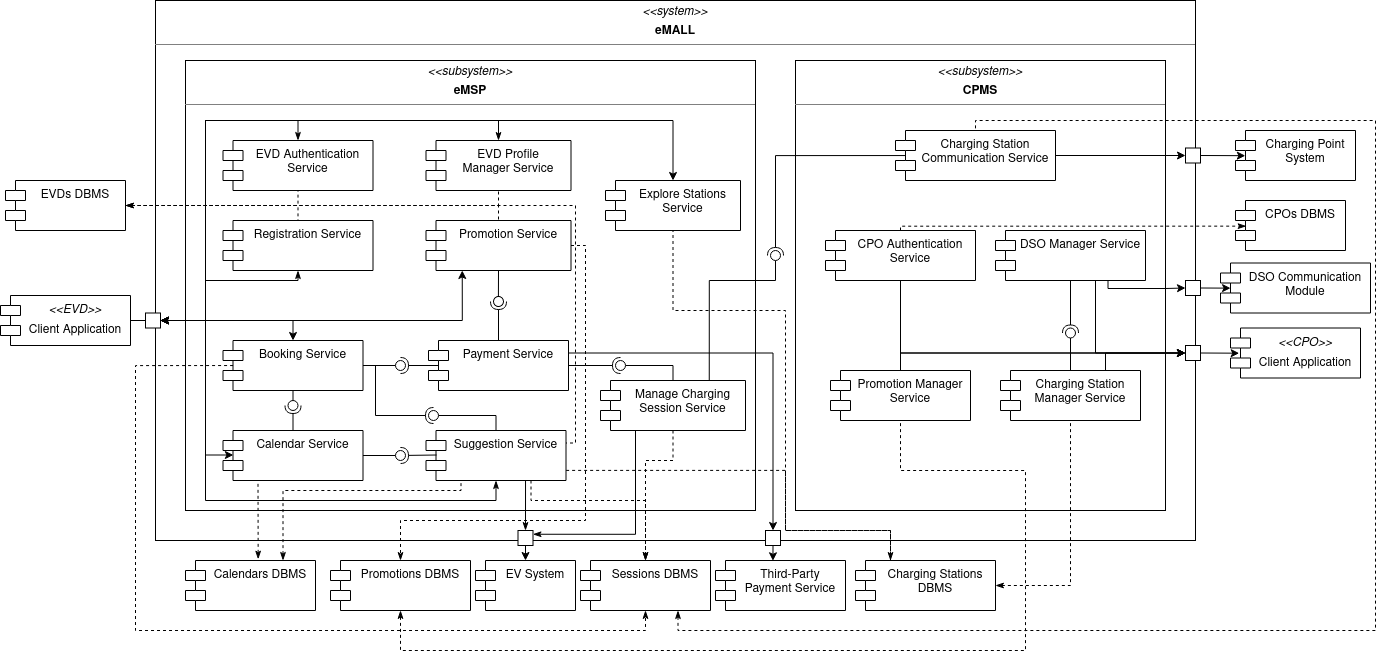
\includegraphics[width=1\linewidth]{ComponentDiagram/component_diagram}
        \caption{Component diagram of the eMALL system.}
        \label{fig: cd}
    \end{center}
\end{figure}

\subsection{Components description}
\label{subsec:components_description}%
The components are:
\begin{itemize}
    \item \textbf{Client Application.} \verb|Client Application| represent the client system used to connect and to communicate
    with \verb|eMALL|.
    \item \textbf{Registration Service.} \verb|Registration Service| handles the process of the creation
    of a new account requested by a new EVD user.
    It communicates with \verb|EVDs DBMS| to save the information about the new created account.
    \item \textbf{EVD Authentication Service.} \verb|EVD Authentication Service| handles the login process requested by an EVD\@.
    To do that, it communicates with \verb|EVDs DBMS| to validate the inserted credentials.
    \item \textbf{EVD Profile Manager Service.} \verb|EVD Profile Manager Service| offers the possibility to query
    the \verb|EVDs DBMS| in order to get requested information.
    In general, it is the service offered to the user to get or update information of the profile.
    So, he communicates with \verb|EVDs DBMS|.
    \item \textbf{Explore Stations Service.} \verb|Explore Stations Service| is the service used by the EVDs to navigate
    into the map of charging station that can be found around user's position.
    To do that, he needs stations position, so it communicates with \verb|Charging Stations DBMS|.
    Furthermore, it communicates also with the external service \verb|Navigator System|, used to elaborate positions
    and to show them into the map.
    \item \textbf{Booking Service.} \verb|Booking Service| is the module used to handle booking requests.
    It communicates with \verb|Sessions DBMS| to save the information about bookings and with \verb|Calendar Service|
    to start the process of insertion of a new activity into EVD's calendar representing the booked reservation.
    \item \textbf{Manage Charging Session Service.} \verb|Manage Charging Session Service| handles the charging session process.
    It allows the EVDs to start and interrupt the session and to pay for the service the user enjoyed.
    Furthermore, it sends to the EVDs notifications about ongoing session status.
    The module communicates with \verb|Charging Station Communication Service| to delegate the communication with the charging point
    where the EVD wants to charge the EV\@.
    As said before, the service offers the EVD the interface to make the payment of the session, so it communicates with
    \verb|Payment Service|.
    After the payment, the module saves the receipt of the session communicating the \verb|Sessions DBMS| module.
    \item \textbf{Promotion Service.} \verb|Promotion Service| offers the EVDs the possibility to activate special promotions
    activated by CPOs.
    To get the list of active promotions, it communicates with \verb|Promotions DBMS|.
    The module communicates also with \verb|EVD Profile Manager Service| to delegate the save of the activation of a special offer into
    the \verb|EVDs DBMS|.
    \item \textbf{Calendar Service.} \verb|Calendar Service| is module that manages EVDs calendar.
    It offers the possibility to visualize the calendar, saved events and their details.
    It also offers the functionality of activity insertion.
    To save all this information, the module communicates with \verb|Calendars DBMS|.
    After a new activity is inserted, \verb|Calendar Service| activates the process offered by \verb|Suggestion Service|
    in order to create suggestion about when and where the EVD should charge the EV\@.
    \item \textbf{Suggestion Service.} \verb|Suggestion Service| communicates with different modules to create suggestions.
    It communicates with:
    \begin{itemize}
        \item \verb|EVDs DBMS| to get user's EV specifications.
        \item \verb|Calendar DBMS| to get EVD's schedule to know precedent events that could affect the research.
        \item \verb|EV System| to get current EV status.
        \item \verb|Charging Stations DBMS| to get positions of the memorized charging stations.
        \item \verb|Navigation System| to calculate the path between the positions defined in the schedule of the EVD,
        and to identify which charging stations can be suggested to the user.
        \item \verb|Sessions DBMS| to get schedules of the charging point, getting in this way their available timeframes,
        and to see if there are other bookings done by the EVD\@.
        \item \verb|Booking Service| to start the booking process after the EVD confirms the received suggestion.
    \end{itemize}
    \item \textbf{Payment Service.} \verb|Payment Service| offers the possibility to pay for a service the EVD enjoyed.
    It communicates with \verb|EVD Profile Manager Service| to get EVD's payment methods.
    Once it has the needed information, it communicates with \verb|Third-Party Payment Service| to make the payment.
    \item \textbf{CPO Authentication Service.} \verb|CPO Authentication Service| handles the login process requested by a CPO\@.
    To do that, it communicates with \verb|CPOs DBMS| to validate the inserted credentials.
    \item \textbf{CPO Profile Manager Service.} \verb|CPO Profile Manager Service| offers the possibility to query
    the \verb|CPOs DBMS| in order to get requested information.
    In general, it is the service offered to the user to get or update information of the profile.
    So, he communicates with \verb|CPOs DBMS|.
    \item \textbf{Charging Station Manager Service.} \verb|Charging Station Manager Service| is the service offered to CPOs
    to manage their charging stations and their charging points.
    One of the functionalities is to plan a maintenance session for a charging station.
    To do that, the module communicates with the \verb|Charging| \verb|Station| \verb|Communication| \verb|Service| module.
    Finally, it communicates with \verb|Charging| \verb|Stations| \verb|DBMS| to store the information.
    \item \textbf{Charging Station Communication Service.} \verb|Charging| \verb|Station| \verb|Communication| \verb|Service| is the module
    that communicates with charging points.
    Messages are exchanged when an EVD starts or ends the charging session or when the CPO plans a maintenance session.
    \item \textbf{Promotion Manager Service.} \verb|Promotion Manager Service| is used by CPOs to manage their promotions.
    The module communicates with \verb|Promotions DBMS| to save or update promotions information.
    \item \textbf{DSO Manager Service.} \verb|DSO Manager Service| is the module aimed for the communication with DSOs.
    To do that, it exchanges messages with the external service \verb|DSO Communication Module|.
    When a CPO decides to change its electricity provider, the module delegates \verb|CPO Profile Manager Service| to
    save the information into the \verb|CPOs DBMS|.
    \item \textbf{EVDs DBMS.} \verb|EVDs DBMS| is the system used to save all the information about EVDs, such as
    credentials, EVs, active promotions.
    \item \textbf{Calendars DBMS.} \verb|Calendars DBMS| is the system used to save all the information about activities
    inserted by EVDs and to save location and hour of a booked charging session.
    In this way, it is easily obtainable by the EVD\@.
    \item \textbf{Sessions DBMS.} \verb|Sessions DBMS| is the system used to save information about bookings
    specifying data that would be useless for the EVD.
    It is also used to save the receipts of the charging sessions done by the EVDs.
    \item \textbf{CPOs DBMS.} \verb|CPOs DBMS| is the system used to save all the information about CPOs, such as credentials,
    company information.
    \item \textbf{Charging Stations DBMS.} \verb|Charging Stations DBMS| is the system used to save the information about
    charging stations and charging points.
    \item \textbf{Promotions DBMS.} \verb|Promotions DBMS| is the system used to save information about promotions
    that have been activated by the CPOs.
    \item \textbf{EV System.} \verb|EV system| is an external service that gives the system the possibility to retrieve
    information about EVDs EV\@.
    \item \textbf{Navigator System.} \verb|Navigator System| is an external service that gives the system the possibility
    to work on positions and elaborate paths between locations.
    \item \textbf{Third-Party Payment Service.} \verb|Third-Party Payment Service| is an external service used to
    make payments communicating with banks or payment sites.
    \item \textbf{Charging Point System.} \verb|Charging Point System| is an external service that represent the software
    running on charging points.
    It is used in the CPOs interactions to manage their charging points.
    \item \textbf{DSO Communication Module.} \verb|DSO Communication Module| is an external service that gives the system
    to communicate with the DSOs in order to get their prices and to enable electricity providing.
\end{itemize}


\section{Deployment View}
\label{sec: deployment_view}%
The following deployment diagram shows how all the components are distributed into different nodes,
highlighting how they communicate with each other. \\
The next paragraphs will go into details about the reasons behind the design choices. \\
The deployment diagram is:
\begin{figure} [H]
    \begin{center}
        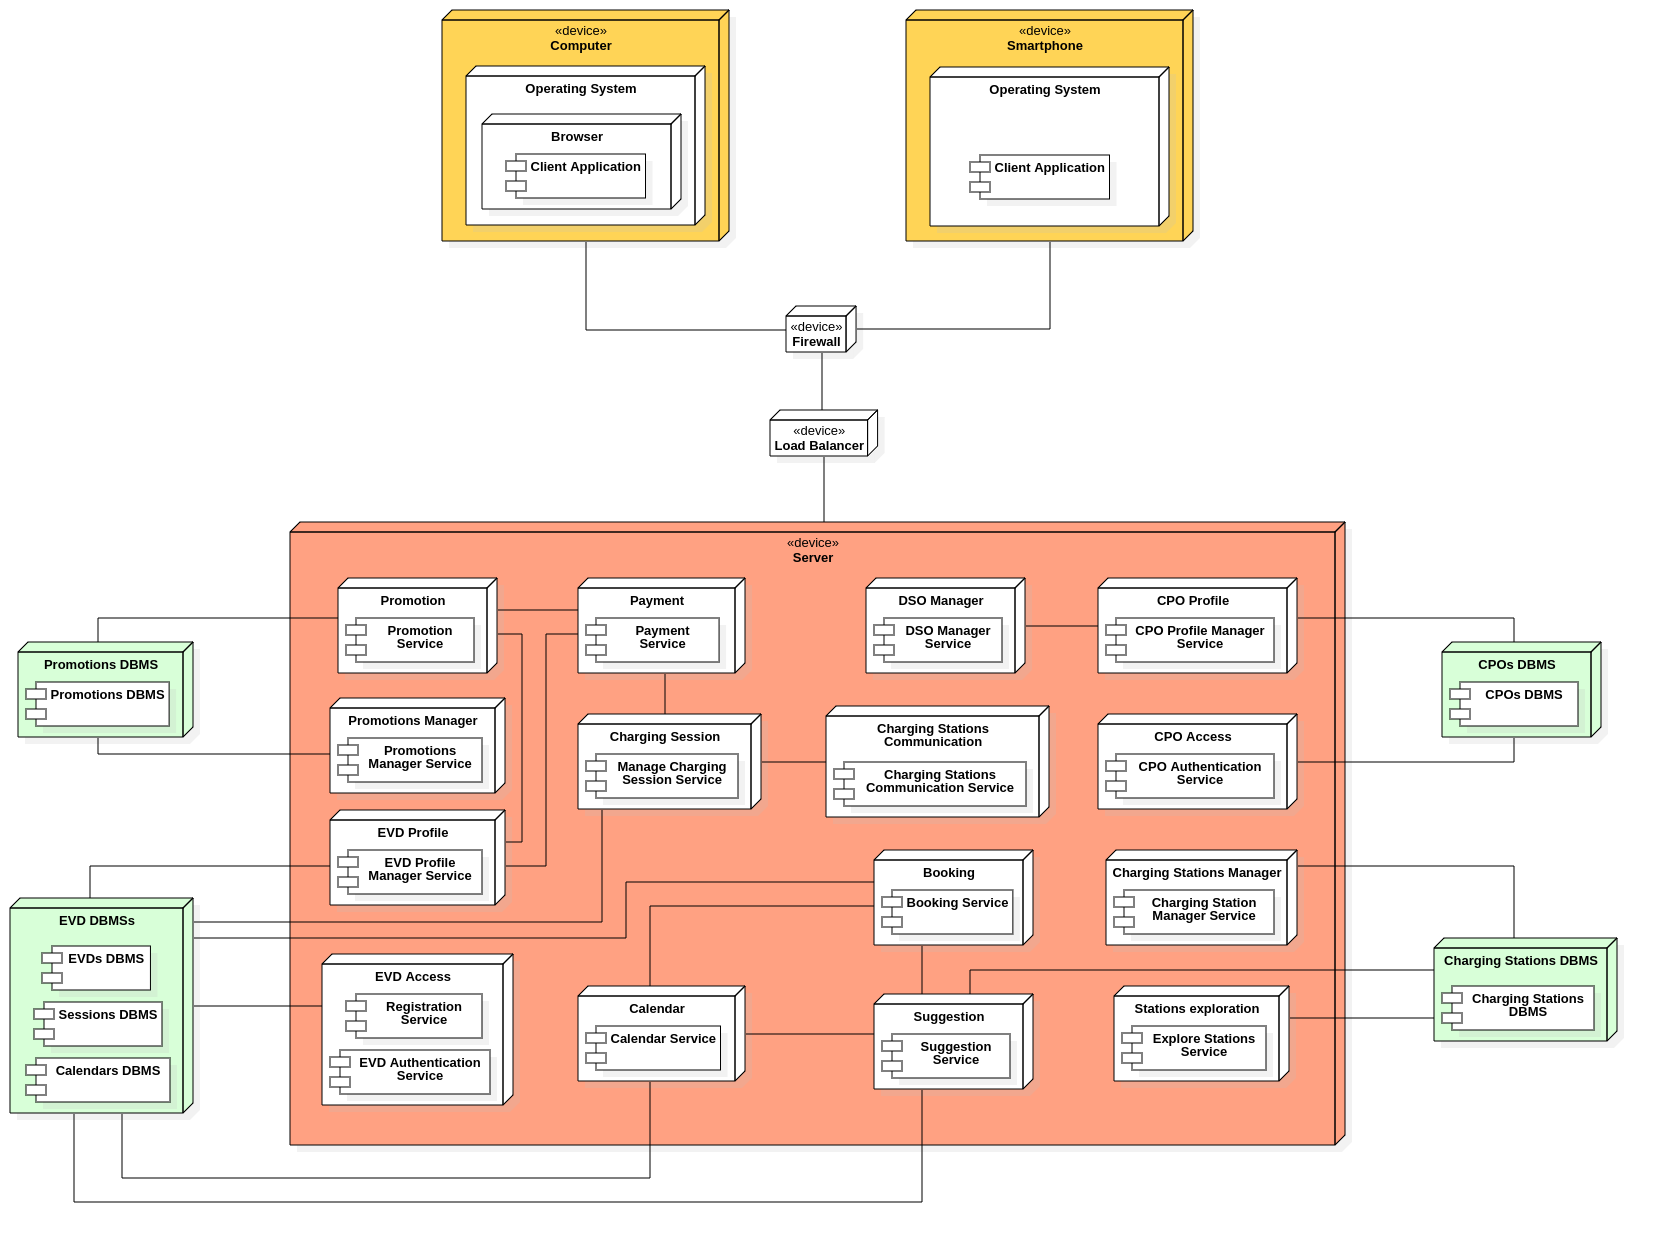
\includegraphics[width=1\linewidth]{DeploymentDiagram/deployment_diagram}
        \caption{Deployment diagram of the eMALL system.}
        \label{fig: depl_diagram}
    \end{center}
\end{figure}

\subsection{Connection to the server}
\label{subsec:connection_to_the_server}%
EVDs and CPOs can access the eMALL system from both PC and smartphones.
In the first case, it is necessary to use a browser to load the system's web page.
In the second case, the client will use the application after downloading it from the smartphone's store (Android or iOS).
When requests are sent to the server, first they pass into the firewall, so to avoid eventual cyberattacks on the system,
then they pass into the load balancer, so to optimize resource usage,
improve performance, and increase the availability of several services.
Requests are now ready to be handled by the eMALL services. \\
It follows the corresponding part from the deployment diagram:
\begin{figure} [H]
    \begin{center}
        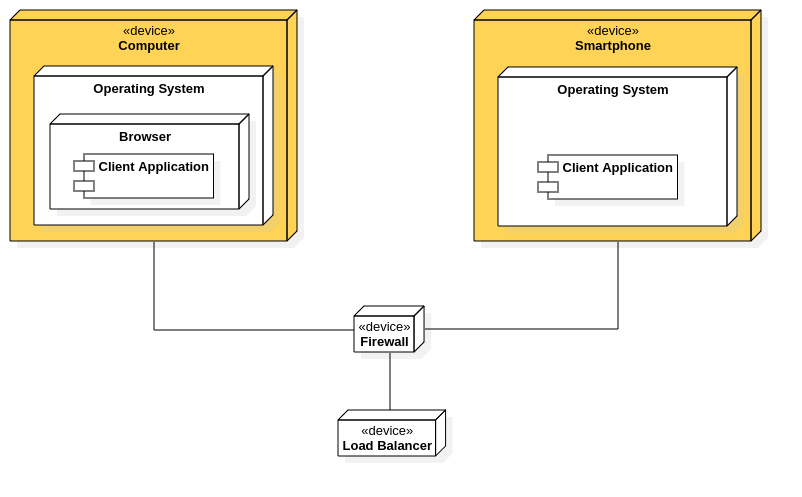
\includegraphics[width=0.7\linewidth]{DeploymentDiagram/connection}
        \caption{Connection to the server diagram.}
        \label{fig: connection}
    \end{center}
\end{figure}

\subsection{Promotions}
\label{subsec:promotions}%
Promotion DBMS is one of the four identified DBMS nodes.
The choice of dividing it from other DBMSs relies on the will to better scale the system.
In this way, it is easier to guarantee the availability of other services that don't work with promotions,
and maintenance sessions are facilitated too.
It has not been grouped with other DBMSs into the same node because Promotions DBMS is also used by CPOs,
so the system needs to guarantee a high level of scalability to assure business functionalities to the companies. \\
It follows the corresponding part from the deployment diagram:
\begin{figure} [H]
    \begin{center}
        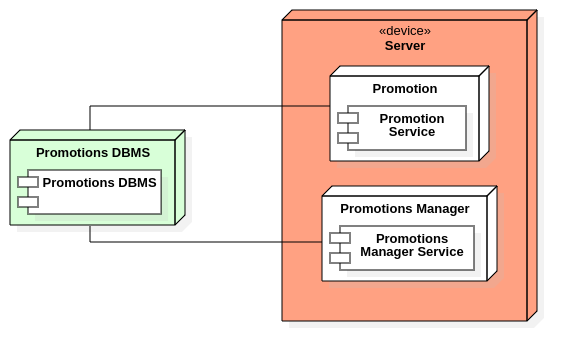
\includegraphics[width=0.6\linewidth]{DeploymentDiagram/promotion}
        \caption{Promotions managing diagram.}
        \label{fig: promotion}
    \end{center}
\end{figure}

\subsection{EVD interactions}
\label{subsec:evd_interactions}%
This section shows how the system communicates with \verb|EVDs DBMS|\@.
We choose to group \verb|EVDs DBMS|, \verb|Sessions DBMS|, and \verb|Calendars DBMS| into the same node because
they all receive requests from the services only in case of interactions with EVDs.
Considering that they don't introduce strict time response requirements,
it was not necessary to insert new physical nodes for the managing of the DBMSs. \\
It follows the corresponding part from the deployment diagram:
\begin{figure} [H]
    \begin{center}
        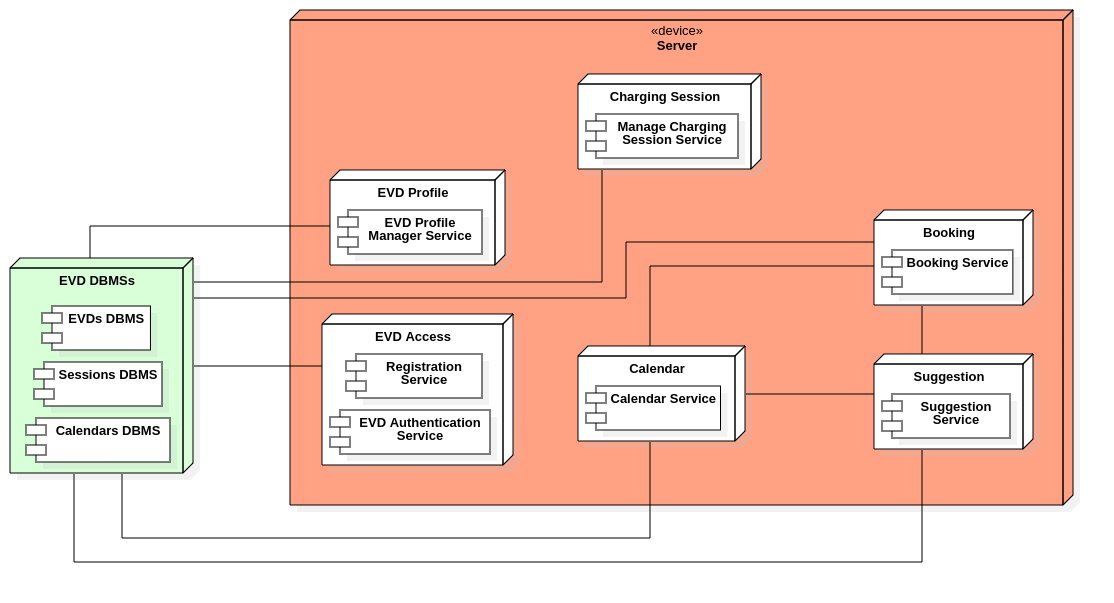
\includegraphics[width=\linewidth]{DeploymentDiagram/EVD_interactions}
        \caption{EVD interactions diagram.}
        \label{fig: evd_interactions}
    \end{center}
\end{figure}

\subsection{CPOs DBMS}
\label{subsec:cpo_dbms}%
The components that communicate with the CPOs DBMS are the Authentication Service and the CPO Profile Manager Service.
When another service needs to get or to update information about a CPO, the request is handled by the CPO Profile node.
The DBMS is used by CPOs, so it is deployed in a single node to better scale the system,
and to guarantee business functionalities to the companies. \\
It follows the corresponding part from the deployment diagram:
\begin{figure} [H]
    \begin{center}
        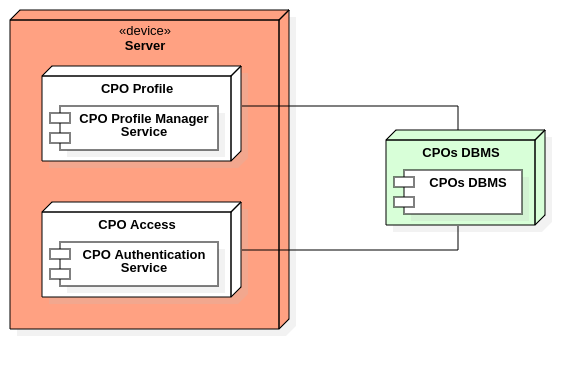
\includegraphics[width=0.6\linewidth]{DeploymentDiagram/CPO_DBMS}
        \caption{CPOs DBMS managing diagram.}
        \label{fig: cpo_dbms}
    \end{center}
\end{figure}

\subsection{Charging stations communication}
\label{subsec:charging_stations_communication}%
Suggestion and Stations exploration nodes read from the DBMS
to get the position of the stations that will be elaborated or shown to the user.
Charging Station Manager Service can also write or update the instances of the DBMS\@.
The DBMS is used by CPOs, so it is deployed in a single node to better scale the system,
and to guarantee business functionalities to the companies. \\
It follows the corresponding part from the deployment diagram:
\begin{figure} [H]
    \begin{center}
        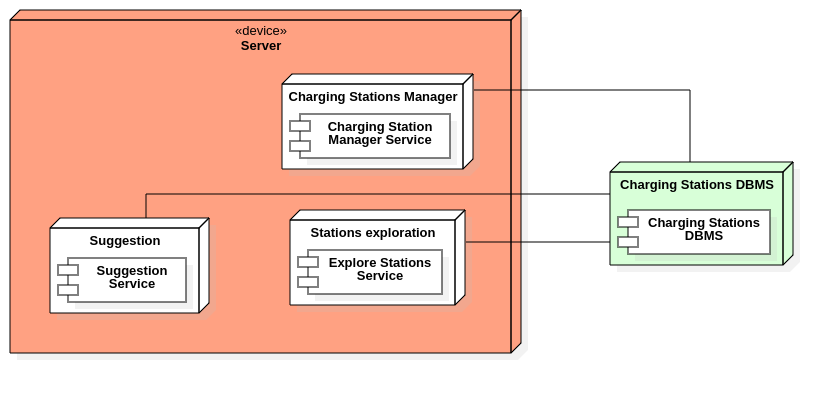
\includegraphics[width=0.85\linewidth]{DeploymentDiagram/charging_stations_communication}
        \caption{Charging stations communication diagram.}
        \label{fig: charing_stations_dbms}
    \end{center}
\end{figure}

\subsection{Services}
\label{subsec:services}%
The section shows all the identified nodes in which services run. \\
Decisions have been made giving particular attention to the concepts of loose coupling and high cohesion.
As explained in Sam Newman's \textit{Building Microservices}, they are defined as follows:
\begin{itemize}
    \item \textbf{Loose coupling.} \textit{When services are loosely coupled, a change to one service should not require a change to another.
    The whole point of a microservice is being able to make a change to one service and deploy it,
        without needing to change any other part of the system.}
    \item \textbf{High Cohesion.} \textit{We want related behavior to sit together, and unrelated behavior to sit elsewhere.
    Making changes in lots of different places is slower, and deploying lots of services at once is risky, both of which we want to avoid.}
\end{itemize}
The following image wants also to highlight the relations between different services, which are direct consequences of the
communication interfaces previously shown in the component diagram.
\begin{figure} [H]
    \begin{center}
        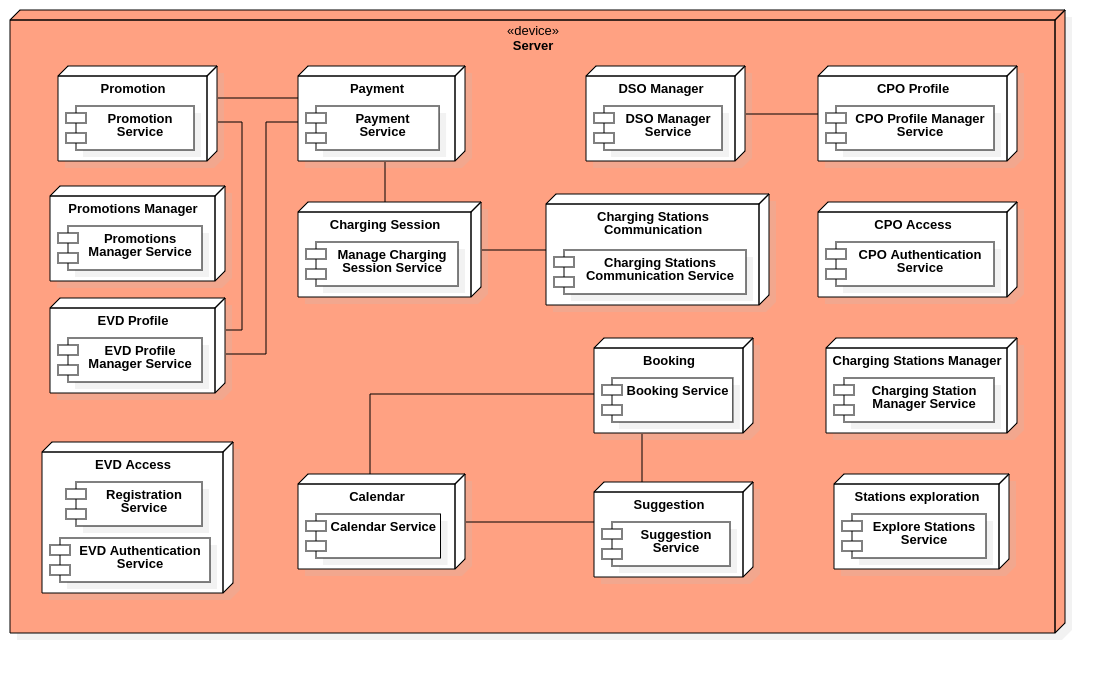
\includegraphics[width=\linewidth]{DeploymentDiagram/server}
        \caption{Server services diagram.}
        \label{fig: services}
    \end{center}
\end{figure}


\section{Runtime View}
\label{sec:runtime_view}%
Here we present the dynamic of our system through sequence diagrams.
We have found the components that communicate with each other to form our system, so now we explain their behaviors.

First, we will present eMALL actions from the point of view of the EVD user, i.e., logging in, booking a charge, managing his profile, etc.
Then, we will present eMALL actions from the point of view of the CPO user, actions that are much more business functionality.
In this section, we hadn't presented all the RASD document use cases because we have decided to focus on the critical part of the system functionalities.

\paragraph{Registered EVD Logs In}
When the EVD - \verb|Client Application| - wants to log in to eMALL, he calls the ``\verb|logIn|'' function from the \verb|EVD| \verb|Authentication| \verb|Service| component.
That component requests the client to display the login form by running the ``\verb|displayLogInForm|'' function, and then it waits for the email and password from the \verb|Client| \verb|Application|.

When the EVD sends this information, the Authentication Service asks the \verb|EVDs| \verb|DBMS| to validate it.
Finished processing the login, the last component returns an ACK message to the \verb|EVD| \verb|Authentication| \verb|Service|, which sends a confirmation or an error to the client.
\begin{figure}[H]
    \begin{center}
        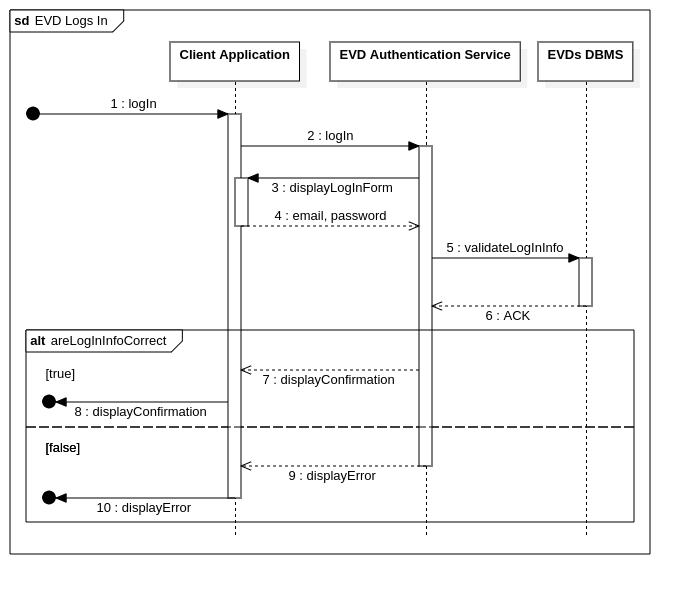
\includegraphics[width=\linewidth]{SequenceDiagrams/EVD Logs In}
        \caption{Registered EVD logs in sequence diagram}
        \label{fig:evd_logs_in}
    \end{center}
\end{figure}

\paragraph{Registered EVD adds an EV}
When the EVD is on his profile page and wants to add a new vehicle to his parking lot, he runs the ``\verb|addVehicle|'' function through the \verb|EVD| \verb|Profile| \verb|Manager| \verb|Service| component.

At first, it asks back to the client to insert the EV information to save in his profile, and then it waits for him.
After the user has sent the information, the component also asks for the nickname to give to the EV\@.
Sending the nickname, the Profile Manager saves the new information by passing them to the \verb|EVDs| \verb|DBMS|\@.
When the DBMS has sent back the ACK message, the \verb|EVD| \verb|Profile| \verb|Manager| \verb|Service| component returns the outcome of the process to the EVD\@.
\begin{figure}[H]
    \begin{center}
        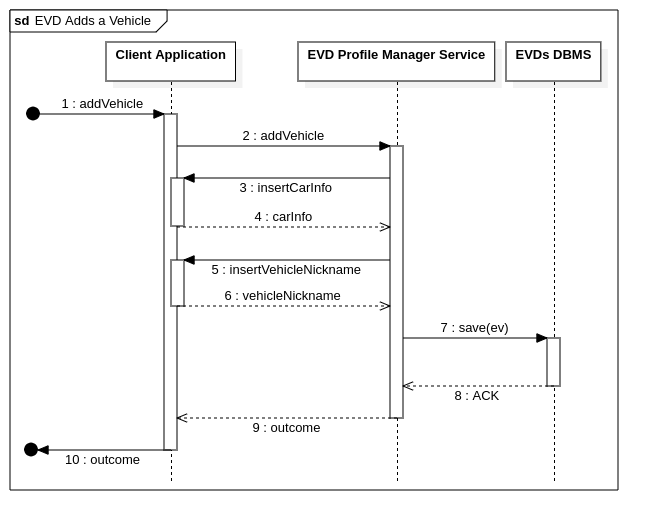
\includegraphics[width=\linewidth]{SequenceDiagrams/EVD Adds a Vehicle}
        \caption{Registered EVD adds an EV sequence diagram}
        \label{fig:evd_adds_vehicle}
    \end{center}
\end{figure}

\paragraph{Registered EVD books a charge}
In eMALL, the EVD can also book a charge in a charging station.
In the sequence diagram, we suppose the \verb|Client| \verb|Application| knows the charging stations he wants to book.
Then, the user calls the ``\verb|bookCharge|'' function of the \verb|Booking| \verb|Service| component, passing the given charging station.

The component needs to know the available timeframes for the charging station, so it waits for the \verb|Sessions| \verb|DBMS| component to process the information.
When it receives the list of timeframes, the \verb|Booking| \verb|Service| asks the user to choose one among them.
Knowing that more than one EVD uses the system, then one timeframe that is at first available might be unavailable when eMALL proceeds with the booking.
To avoid it, the \verb|Booking| \verb|Service| asks for the \verb|Sessions| \verb|DBMS| to check the availability of the chosen timeframe and to lock it if so by calling the ``\verb|isTimeframeAvailable|'' function.

Once the chosen timeframe is locked, the component asks the EVD to confirm the booking - ``\hyperlink{evdconfirmsbooking}{EVD Confirms the Booking}'' sequence diagram.
In the end, the system sends the outcome of the process to the \verb|EVD Client Application|.
\begin{figure}[H]
    \begin{center}
        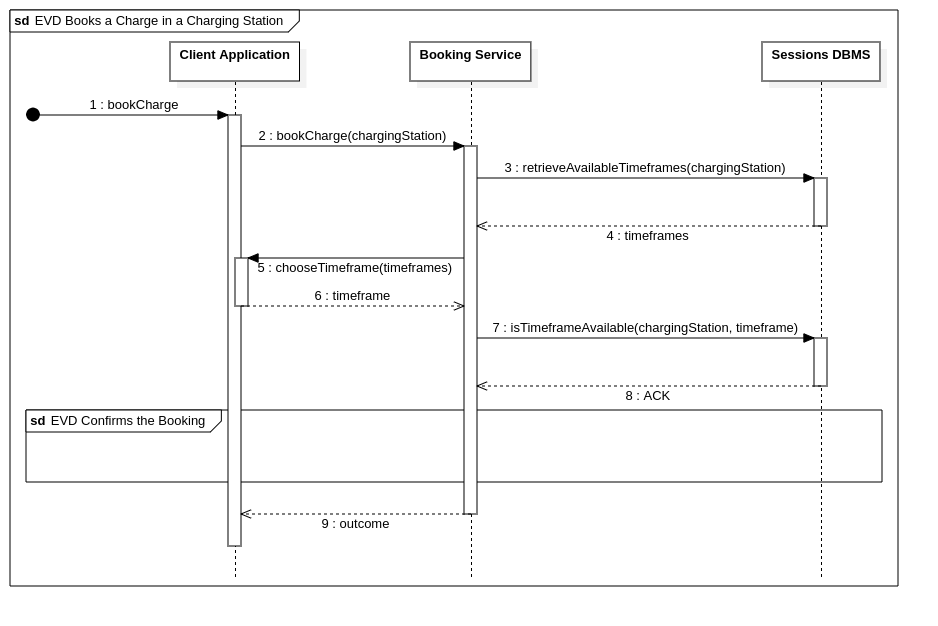
\includegraphics[width=\linewidth]{SequenceDiagrams/EVD Books a Charge in a Charging Station}
        \caption{Registered EVD books a charge sequence diagram}
        \label{fig:evd_books_charge_charging_station}
    \end{center}
\end{figure}

\paragraph{\texorpdfstring{\protect\hypertarget{evdconfirmsbooking}{Registered EVD confirms the booking}}{}}
Our system always asks the client to confirm a booking before saving it, so the \verb|Booking| \verb|Service| component receives the client, the charging station where he wants to book, and the timeframe to reserve for the client.
At first, it asks the EVD to confirm the booking and waits for his reply.
Given the confirmation, the \verb|Booking| \verb|Service| runs the ``\verb|addSession|'' function of \verb|Sessions| \verb|DBMS| to add the new booking to the database and orders to the \verb|Calendar| \verb|Service| to add it to the calendar.
After the \verb|Calendar| \verb|Service| has run the ``\verb|saveActivity|'' function of \verb|Calendars| \verb|DBMS|, \verb|Booking| \verb|Service| returns the outcome to the caller.
\begin{figure}[H]
    \begin{center}
        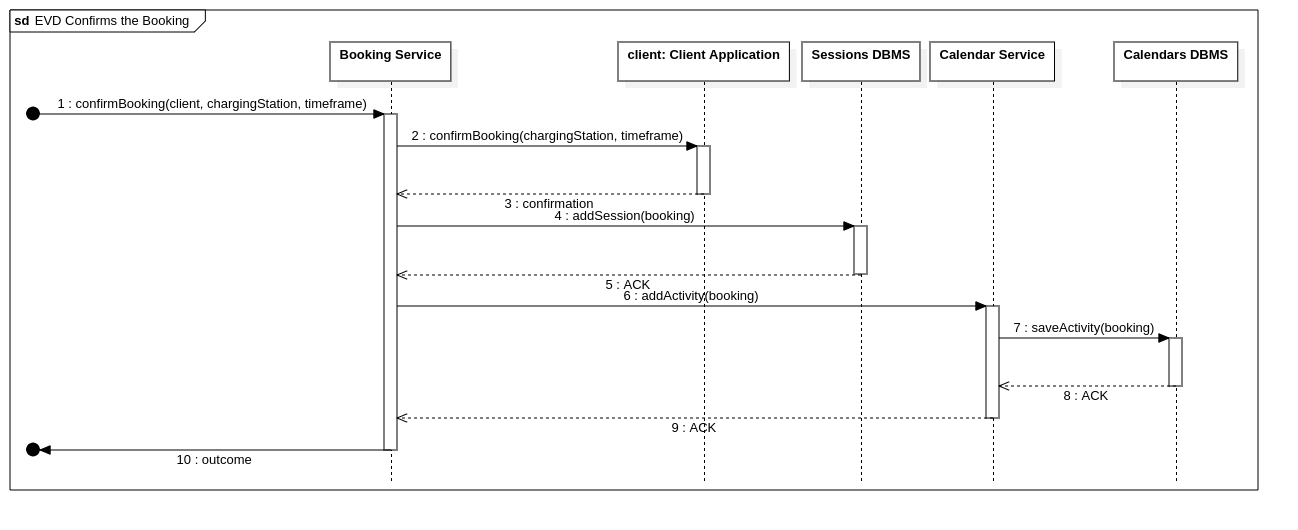
\includegraphics[width=\linewidth]{SequenceDiagrams/EVD Confirms the Booking}
        \caption{Registered EVD confirms the booking sequence diagram}
        \label{fig:evd_confirms_booking}
    \end{center}
\end{figure}

\paragraph{Registered EVD consults a specific promotion that can be redeemed}
An EVD might want to redeem an available promotion in eMALL through his page.
He has to call the ``\verb|redeemPromotion|'' function from the \verb|Promotion| \verb|Service| component, which retrieves all the promotions by running the get function of the list of promotions from the \verb|Promotions| \verb|DBMS|\@.
When the \verb|Promotion| \verb|Service| has received the list, it asks the user to select which promotion he wants to redeem and then asks for a confirmation for its activation.

If the user has decided to proceed with the activation, \verb|Promotion| \verb|Service| initializes the payment by calling the ``\verb|pay|'' function from the \verb|Payment| \verb|Service| component - ``\hyperlink{evdmakespayment}{EVD Makes a Payment}'' sequence diagram.
When the payment successfully ends, the activation process runs through the \verb|EVD| \verb|Profile| \verb|Manager| \verb|Service| component by calling the ``\verb|activate|'' function that receives the paid promotion and the client in input.
The Profile Manager calls the counterpart ``\verb|activate|'' function from the \verb|EVDs| \verb|DBMS|\@.
\begin{figure}[H]
    \begin{center}
        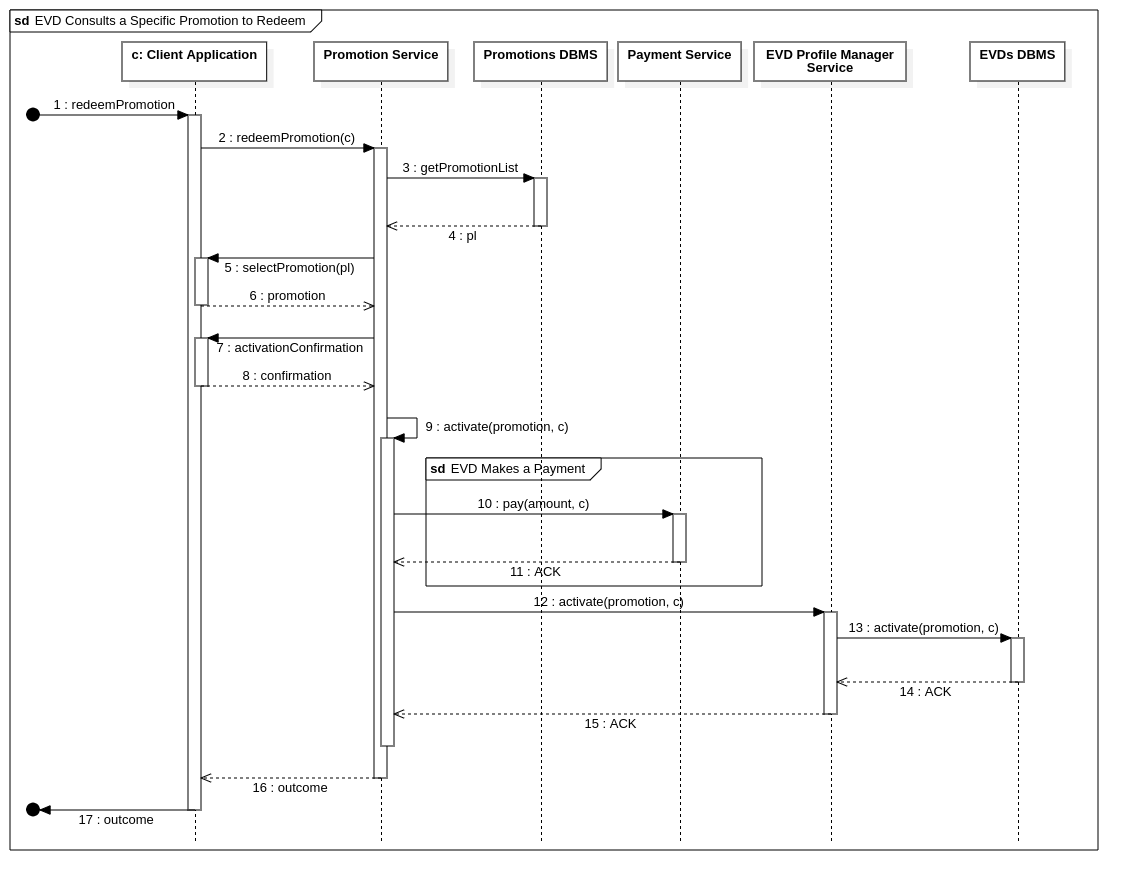
\includegraphics[width=\linewidth]{SequenceDiagrams/EVD Consults a Specific Promotion to Redeem}
        \caption{Registered EVD consults a specific promotion that can be redeemed sequence diagram}
        \label{fig:evd_consults_specific_promotion_to_redeem}
    \end{center}
\end{figure}

\paragraph{Registered EVD charges his EV}
Now we explain how a charging process evolves in eMALL\@.
At first, we need the EVD to call the function ``\verb|startChargeEV|'' from the \verb|Manage| \verb|Charging| \verb|Session| \verb|Service| component to verify that the current user has booked a charging session.
The service calls so the ``\verb|validateClient|'' from the \verb|Sessions| \verb|DBMS| because it is the only one that can retrieve this information.

The timeframe is not necessary because the system checks at the current time.
If the EVD has booked, the service requests to unlock the charging point to the \verb|Charging| \verb|Station| \verb|Communication| \verb|Service|, which delegates the process to the \verb|Charging| \verb|Point| \verb|System|.
Once the charging point is unlocked, the \verb|Manage| \verb|Charging| \verb|Session| \verb|Service| asks the user to connect his EV and confirm the start of the charging process.

When the EVD confirms, the service asks the \verb|Charging| \verb|Session| \verb|Communication| \verb|Service| to start charging, which delegates to the \verb|Charging| \verb|Point| \verb|System|.
Then, we have a loop sequence where the user asks indirectly for information from the \verb|Charging| \verb|Point| \verb|System| to see the status of his EV's battery.
When the EVD decides to stop the charging process, he communicates it to the \verb|Manage| \verb|Charging| \verb|Session| \verb|Service|, which delegates the decision to the \verb|Charging| \verb|Session| \verb|Communication| \verb|Service|, which orders to stop charging to the \verb|Charging| \verb|Point| \verb|System|.
Finally, the \verb|Manage| \verb|Charging| \verb|Session| \verb|Service| initializes the payment - \hyperlink{evdmakespayment}{EVD Makes a Payment} sequence diagram - and calls the ``\verb|save|'' function from the \verb|Sessions| \verb|DBMS| to save the EVD session.
\begin{figure}[H]
    \begin{center}
        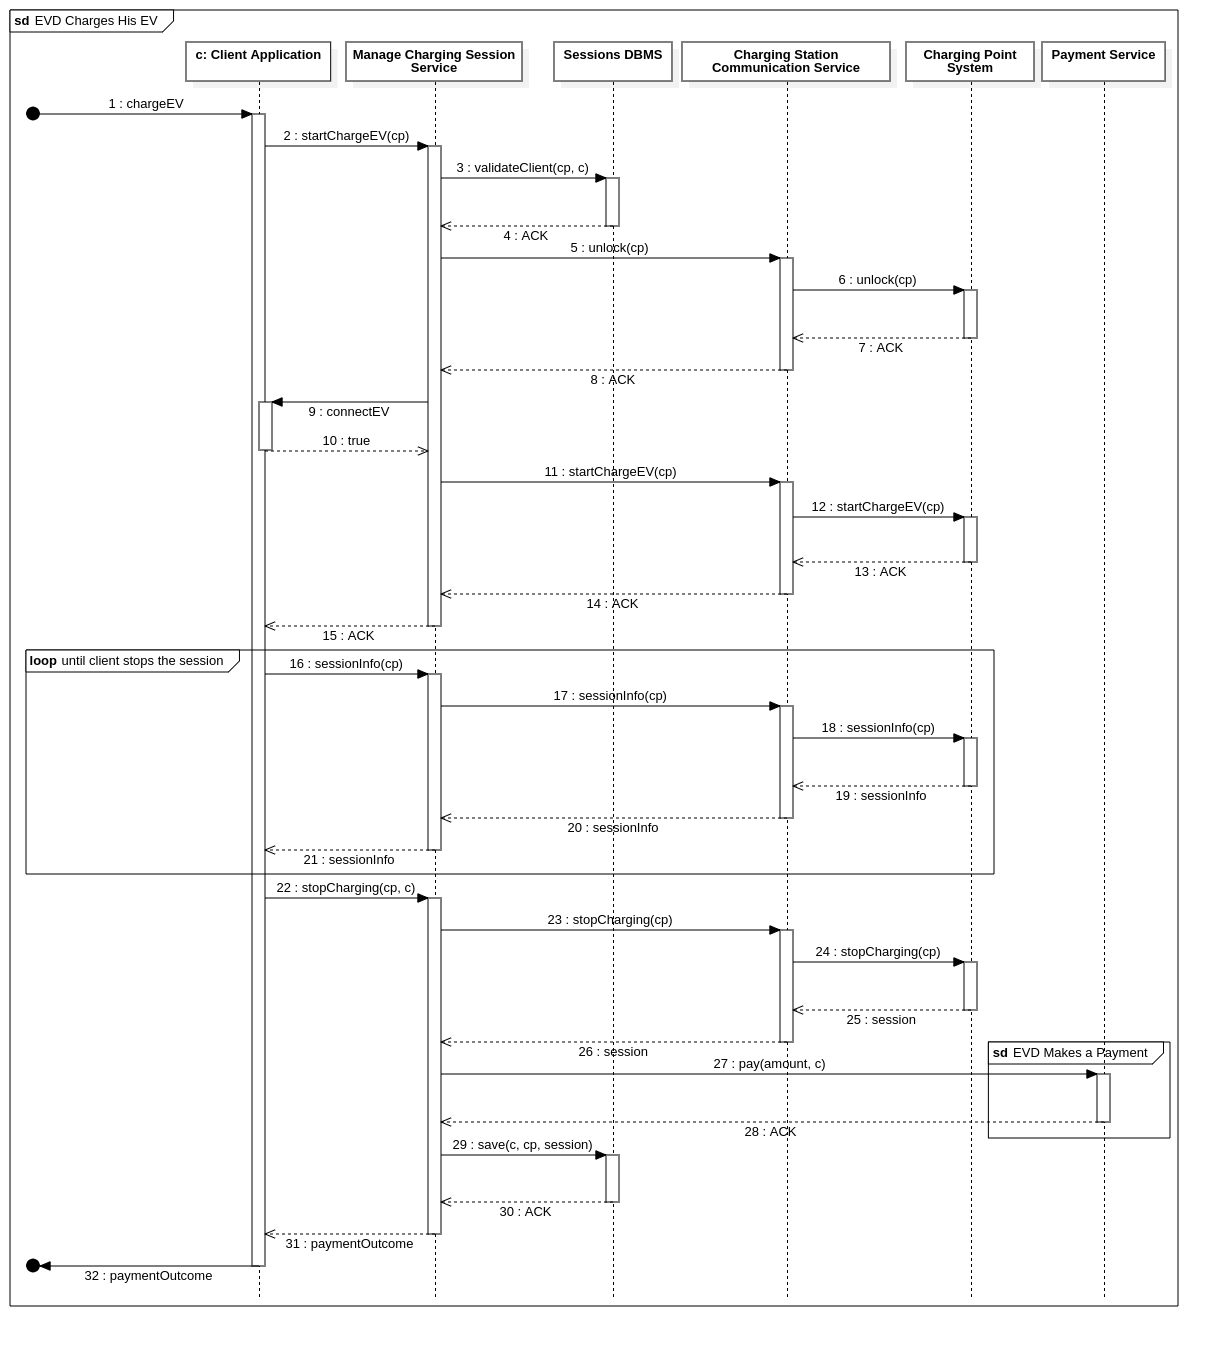
\includegraphics[width=\linewidth]{SequenceDiagrams/EVD Charges His EV}
        \caption{Registered EVD charges his EV sequence diagram}
        \label{fig:evd_charges_his_ev}
    \end{center}
\end{figure}

\paragraph{\texorpdfstring{\protect\hypertarget{evdmakespayment}{Registered EVD makes a payment}}{}}
When an EVD has to pay, the \verb|Payment| \verb|Service| receives a call with the amount to pay from a client and the client himself in input.
The service asks the \verb|EVD| \verb|Profile| \verb|Manager| \verb|Service| to select a payment method for the given EVD\@.
The Profile Manager asks the \verb|EVDs| \verb|DBMS| for the user's payment methods by calling the ``\verb|getPaymentMethods|'' function and returns the obtained list to the caller.
Finally, the \verb|Payment| \verb|Service| runs the ``\verb|pay|'' function from the \verb|Third-party| \verb|Payment| \verb|Service| with the amount to pay in input.
\begin{figure}[H]
    \begin{center}
        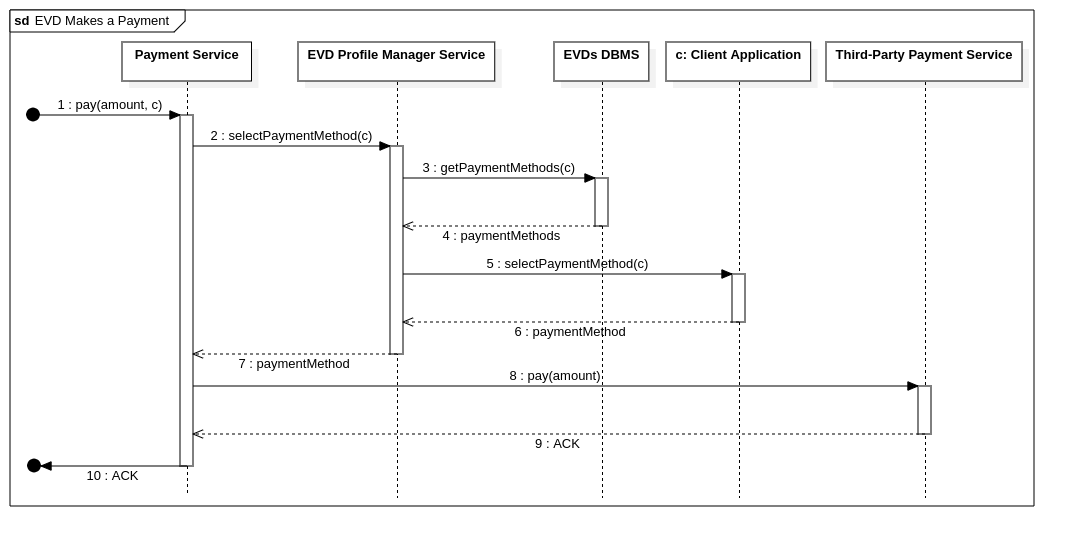
\includegraphics[width=\linewidth]{SequenceDiagrams/EVD Makes a Payment}
        \caption{Registered EVD makes a payment sequence diagram}
        \label{fig:evd_makes_payment}
    \end{center}
\end{figure}

\paragraph{Registered EVD adds a new activity into the calendar and receives suggestions about charging schedule}
When the EVD wants to add a new activity to his calendar, he first opens the calendar section by calling the ``\verb|openCalendar|'' function from the \verb|Calendar| \verb|Service| component, which delegates the call to \verb|Calendars| \verb|DBMS|\@.

Once the user has received the calendar, he can insert the new activity by requesting a form to the \verb|Calendar| \verb|Service| through the ``\verb|insertNewActivity|'' function call.
When the user fills out the form, he sends it to the \verb|Calendar| \verb|Service|, which calls the ``\verb|validateActivity|'' function from the \verb|Calendars| \verb|DBMS| and then the ``\verb|saveActivity|'' function from the same DBMS component.

Finally, the service initializes asynchronously the function ``\verb|findBestSchedule|,'' which computes the best path in reaching the different appointments of the user depending on the battery status of the EV, its capacity, and energy costs.
The call is asynchronous because the service is not essential for the EVD\@.
If the \verb|Suggestion| \verb|Service| component is down, eMALL has to work without it and allow the users to add new activities to their calendars.
\begin{figure}[H]
    \begin{center}
        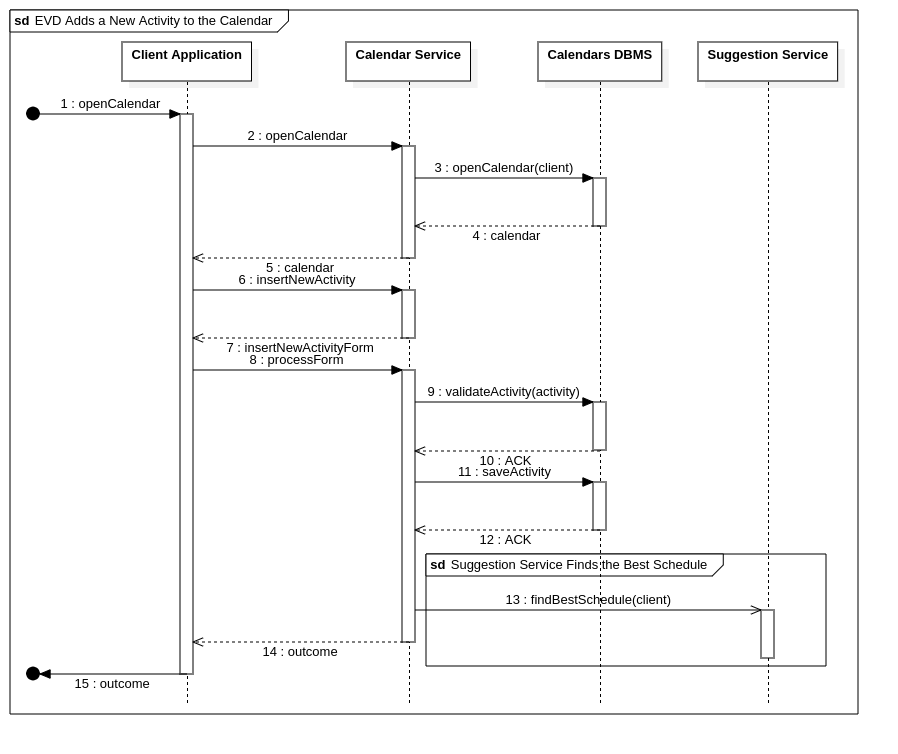
\includegraphics[width=\linewidth]{SequenceDiagrams/EVD Adds a New Activity to the Calendar}
        \caption{Registered EVD adds a new activity into the calendar and receives suggestions about charging schedule sequence diagram}
        \label{Registered EVD adds a new activity into the calendar and receives suggestions about charging schedule sequence diagram}
    \end{center}
\end{figure}

\paragraph{CPO logs in}
In eMALL, when a CPO wants to log in, he calls the function ``\verb|logInCPO|'' from the \verb|CPO| \verb|Authentication| \verb|Service| component, which calls back the ``\verb|insertInfo|'' function from the \verb|Client| \verb|Application| to retrieve the essential information for the CPO identification, i.e., ID, email, and password.
Once the CPO has sent the information, the Authentication Service runs the ``\verb|validateAccount|'' function from the \verb|CPOs| \verb|DBMS|\@.
If the CPO operator has inserted the correct credentials, he will enter his homepage.
\begin{figure}[H]
    \begin{center}
        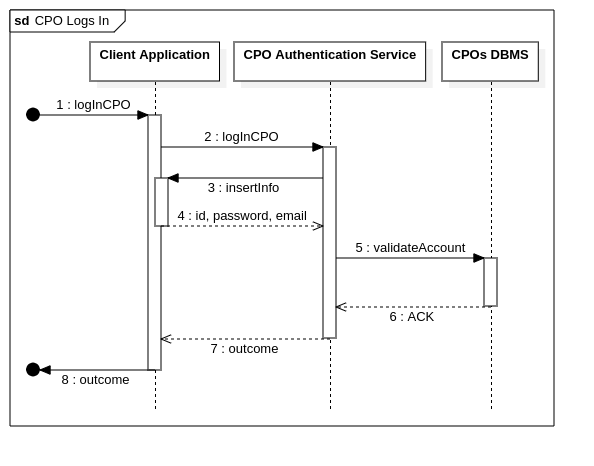
\includegraphics[width=\linewidth]{SequenceDiagrams/CPO Logs In}
        \caption{CPO logs in sequence diagram}
        \label{cpo_logs_in}
    \end{center}
\end{figure}

\paragraph{CPO sets a fee}
From his homepage, a CPO might want to change the fees of his charging stations.
When he has decided which charging station, he calls the ``\verb|setFee|'' function from the \verb|Charging| \verb|Station| \verb|Manager| \verb|Service| component, which asks the user to insert the new fee to set to the given charging station.
Once the CPO has specified the new fee, the Charging Station Manager runs the ``\verb|updateFee|'' function from the \verb|Charging| \verb|Stations| \verb|DBMS|, which replaces the old fee value with the new one in input.
\begin{figure}[H]
    \begin{center}
        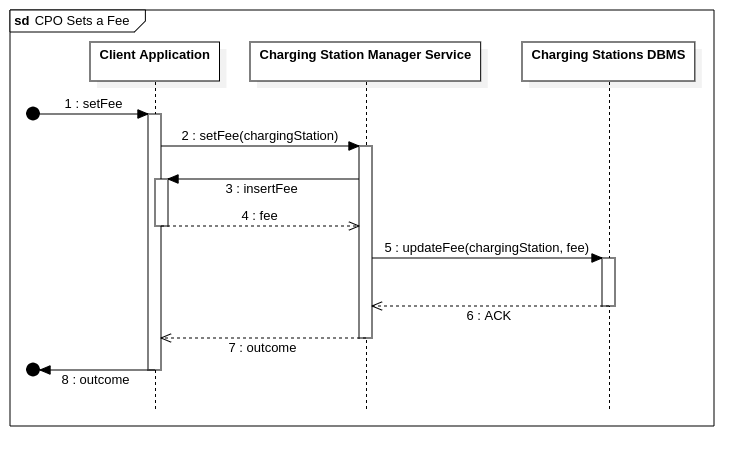
\includegraphics[width=\linewidth]{SequenceDiagrams/CPO Sets a Fee}
        \caption{CPO sets a fee sequence diagram}
        \label{cpo_sets_fee}
    \end{center}
\end{figure}

\paragraph{CPO adds a charging station}
From his homepage, a CPO can add new charging stations to his profile, so he calls the ``\verb|addChargingStation|'' function from the \verb|Charging| \verb|Station| \verb|Manager| \verb|Service| component.
The service asks the \verb|Client| \verb|Application| to insert the location of the new charging station, its status, the charging costs, and the charging points with their information.
For each piece of information, the service waits for the CPO to reply before proceeding with the new request.
Once the service has received all the information, it passes them to the validate function called from the \verb|Charging| \verb|Stations| \verb|DBMS|\@.
\begin{figure}[H]
    \begin{center}
        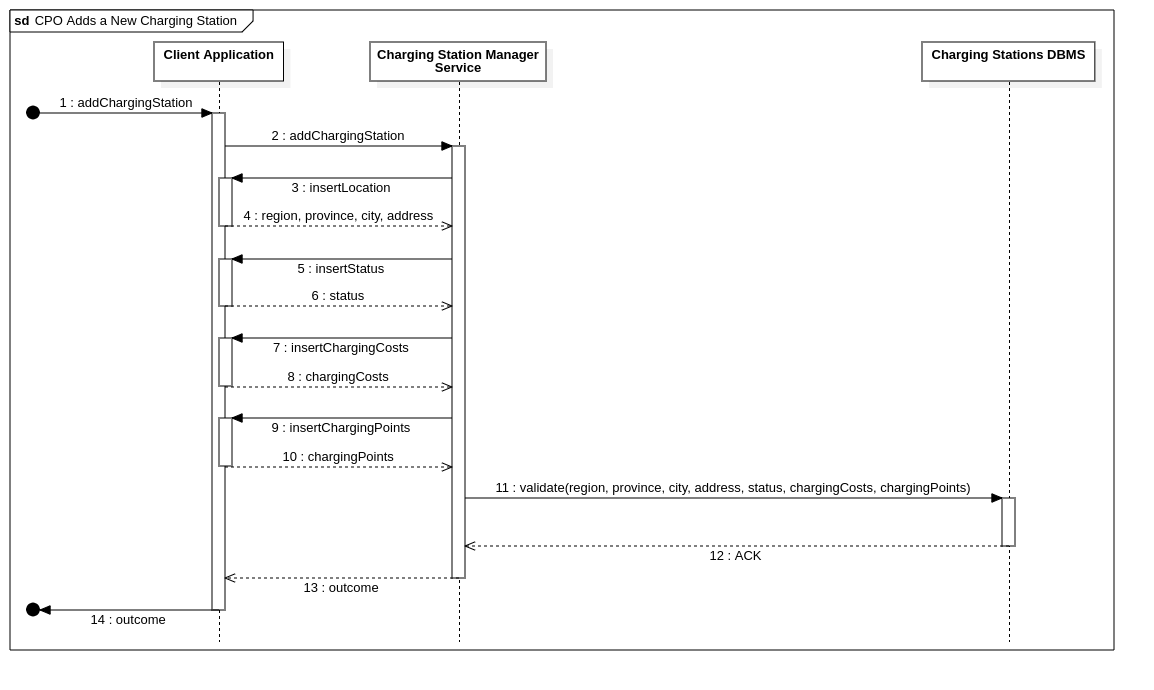
\includegraphics[width=\linewidth]{SequenceDiagrams/CPO Adds a New Charging Station}
        \caption{CPO adds a charging station sequence diagram}
        \label{cpo_adds_new_charging_station}
    \end{center}
\end{figure}

\paragraph{CPO adds a charging point}
A CPO can also add new charging points to an existing charging station.
When he chooses this operation, he calls the ``\verb|addChargingPoint|'' function from the \verb|Charging| \verb|Station| \verb|Manager| \verb|Service| component, which asks the \verb|Client| \verb|Application| to enter the charging station where the new charging point has to be added and then the information of the charging point itself.
Once the service has received all the information, it passes them to the validate function called from the \verb|Charging| \verb|Stations| \verb|DBMS|\@.
\begin{figure}[H]
    \begin{center}
        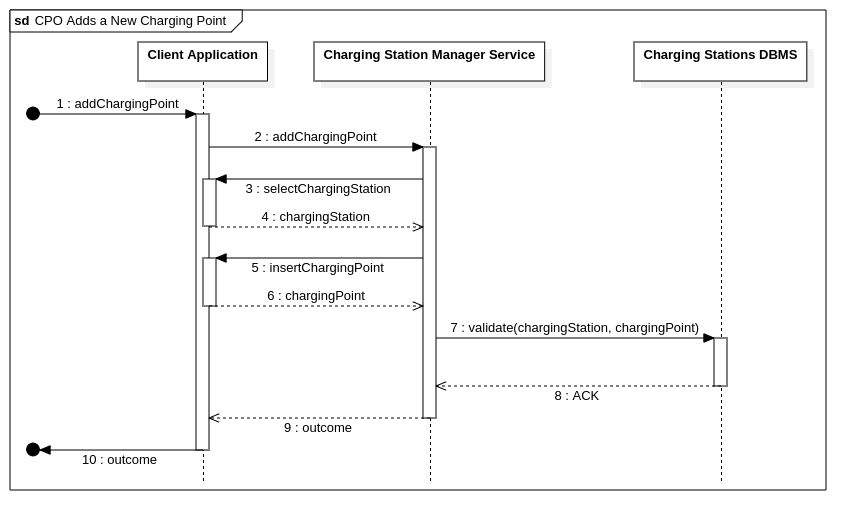
\includegraphics[width=\linewidth]{SequenceDiagrams/CPO Adds a New Charging Point}
        \caption{CPO adds a charging point sequence diagram}
        \label{cpo_adds_new_charging_point}
    \end{center}
\end{figure}

\paragraph{CPO changes the metadata of a charging point}
When a CPO wants to edit the metadata of charging points, he calls the ``\verb|updateMetadataChargingPoint|'' from the \verb|Charging| \verb|Station| \verb|Manager| \verb|Service| component with the given charging station in input.
At first, the service asks the \verb|Client| \verb|Application| to select the charging point to edit, so it calls the ``\verb|editMetadataChargingPoint|'' function from the \verb|Client| \verb|Application| that allows the CPO to edit the charging point information.
Once the user has filled out the form, the function returns the new charging point to the Charging Station Manager, which calls the update function with the charging station, the old charging point, and the up-to-date charging point from the \verb|Charging| \verb|Stations| \verb|DBMS|\@.
\begin{figure}[H]
    \begin{center}
        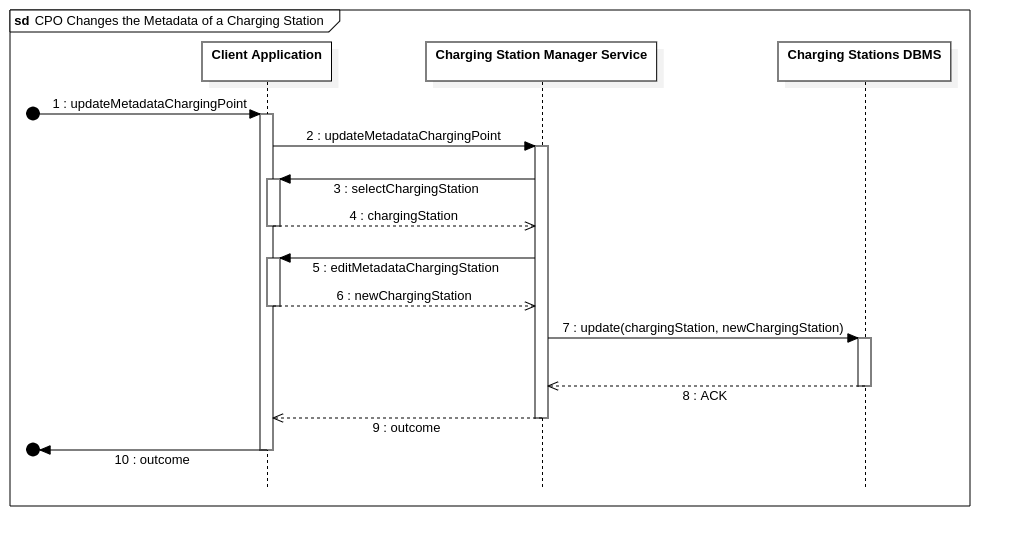
\includegraphics[width=\linewidth]{SequenceDiagrams/CPO Changes the Metadata of a Charging Station}
        \caption{CPO changes the metadata of a charging point sequence diagram}
        \label{cpo_changes_metadata_of_charging_point}
    \end{center}
\end{figure}

\paragraph{CPO activates a promotion}
The CPO can define promotions for the EVD\@.
At first, the CPO calls the ``\verb|activatePromotion|'' function from the \verb|Promotion| \verb|Manager| \verb|Service| component, which calls back the ``\verb|definePromotionFeatures|'' from the \verb|Client| \verb|Application|.
The function, as the name suggests, allows the CPO to define the features of the new promotion.
The form is sent to the caller when filled out.
The Promotion Manager processes the result and, if it's correct, calls the function ``\verb|save|'' with the promotion in input from the \verb|Promotions| \verb|DBMS|\@.
If the store is successful, the service calls the ``\verb|initialize|'' function to make the promotion available to EVDs\@.
\begin{figure}[H]
    \begin{center}
        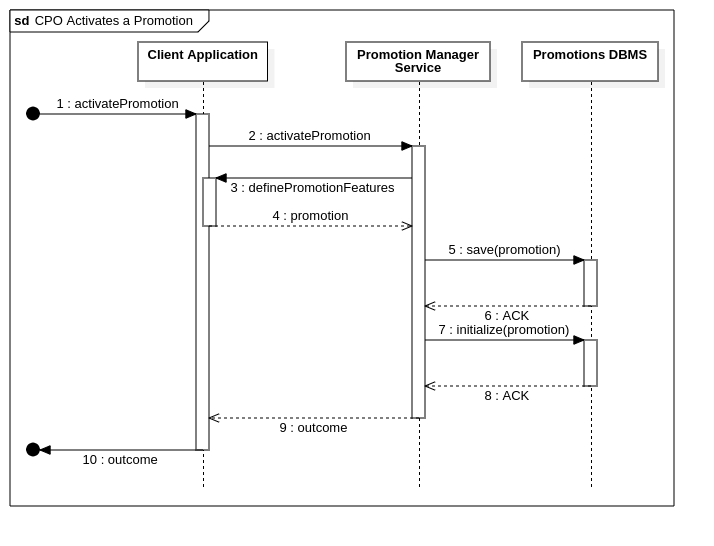
\includegraphics[width=\linewidth]{SequenceDiagrams/CPO Activates a Promotion}
        \caption{CPO activates a promotion sequence diagram}
        \label{cpo_activates_promotion}
    \end{center}
\end{figure}

\paragraph{CPO plans a maintenance session for a charging station}
A CPO can plan maintenance sessions for his charging station, so here we describe the sequence diagram of the planning process.
At first, the CPO calls the ``\verb|planMaintenanceSession|'' function from the \verb|Charging| \verb|Station| \verb|Manager| \verb|Service| component with the charging station in input.
The service asks the user to fill out the form for the date and hour of the planned maintenance.
Once the CPO returns the form, the Charging Station Manager calls the ``\verb|planMaintenance|'' function from the \verb|Charging| \verb|Station| \verb|Communication| \verb|Service|, which delegates the job to the \verb|Charging| \verb|Point| \verb|System|.
The function notifies the \verb|Charging| \verb|Point| \verb|System| that the charging points of a given charging station will be unavailable on a particular date.
When the Charging Station Manager receives the success notification of the alert, it saves the information into the \verb|Charging| \verb|Stations| \verb|DBMS| by calling the ``\verb|savePlannedMaintenance|'' function with the charging station, date, and hour in input.
\begin{figure}[H]
    \begin{center}
        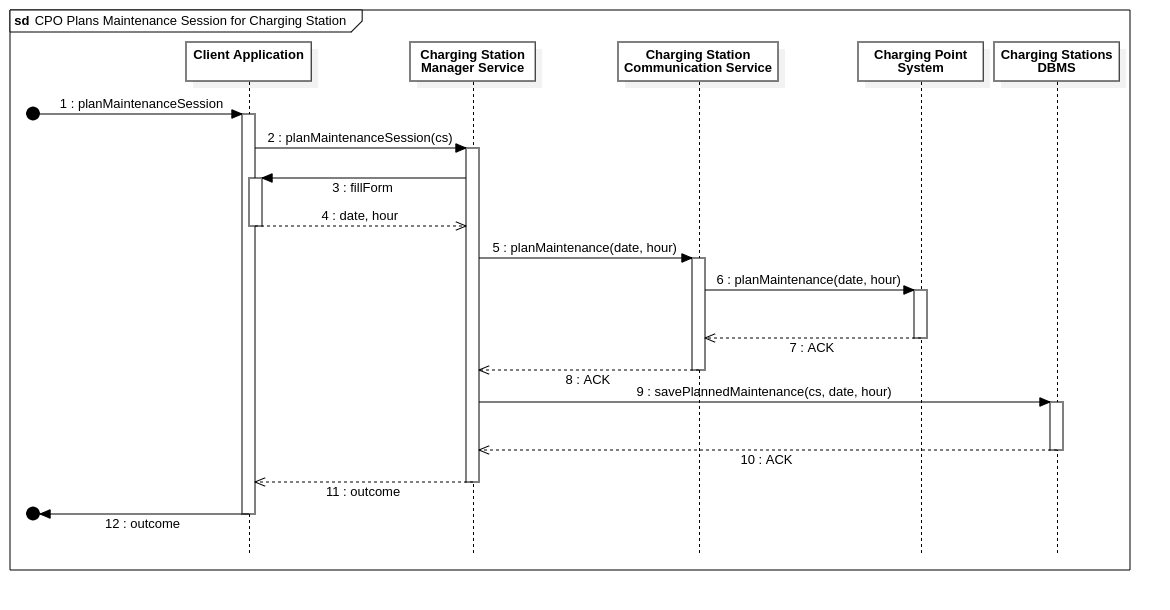
\includegraphics[width=\linewidth]{SequenceDiagrams/CPO Plans Maintenance Session for Charging Station}
        \caption{CPO plans a maintenance session for a charging station sequence diagram}
        \label{cpo_plans_maintenance_session_for_charging_station}
    \end{center}
\end{figure}

\paragraph{CPO decides the DSO from which acquire energy}
A CPO can edit his energy provider - DSO - from his homepage.
At first, he calls the ``\verb|setDSOAcquireEnergy|'' function from the \verb|DSO| \verb|Manager| \verb|Service| with the CPO's identifier in input.
The DSO Manager orders the \verb|DSO| \verb|Communication| \verb|Module| to return the list of all the DSOs available in eMALL\@.
When the list is ready, the DSO Manager asks the client to select the DSO from the list, and then it runs the ``\verb|activateDSO|'' function of the \verb|DSO| \verb|Communication| \verb|Module|, which alerts the DSO that a new CPO will acquire energy from it.
After the alert, the service calls the ``\verb|update|'' function from the \verb|CPO| \verb|Profile| \verb|Manager| \verb|Service|, which delegates to the counterpart ``\verb|update|'' function of the \verb|CPOs| \verb|DBMS| to store the new relationship.
The process ends by notifying the \verb|Client| \verb|Application| about the successful ending of the operation.
\begin{figure}[H]
    \begin{center}
        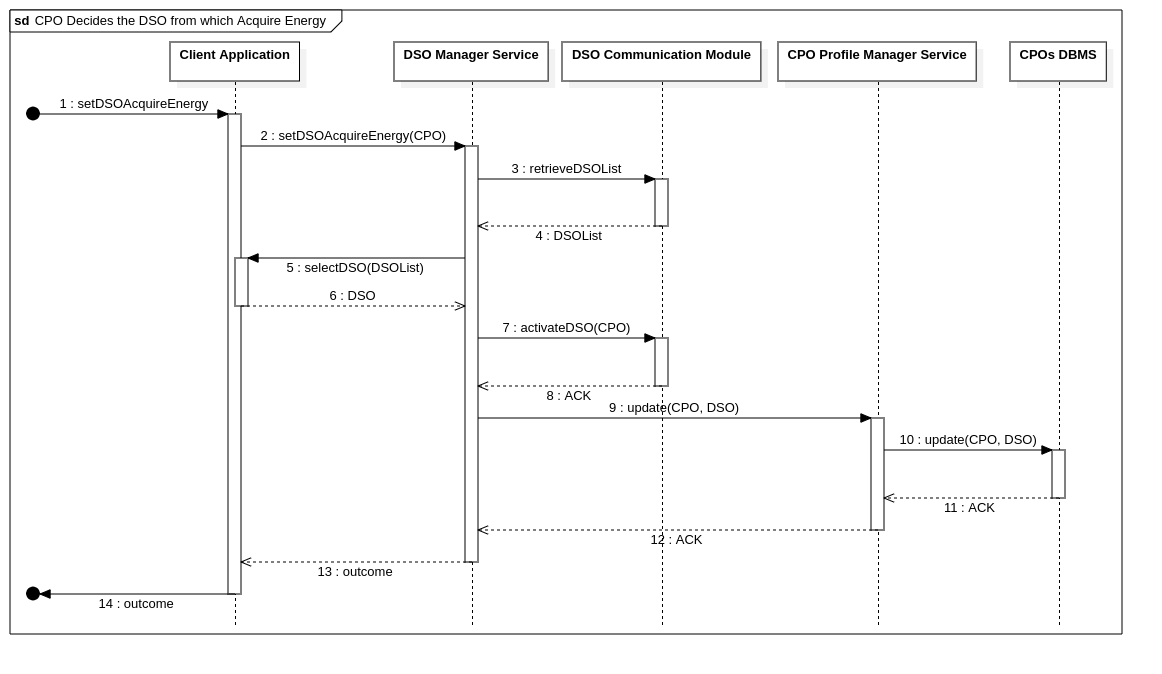
\includegraphics[width=\linewidth]{SequenceDiagrams/CPO Decides the DSO from which Acquire Energy}
        \caption{CPO decides the DSO from which acquire energy sequence diagram}
        \label{cpo_decides_dso_from_which_acquire_energy}
    \end{center}
\end{figure}


\section{Component Interfaces}
\label{sec: component_interfaces}%


\section{Selected Architectural Styles and Patterns}
\label{sec: patterns}%


\section{Other Design Decisions}
\label{sec: other_design_decisions}%



    \chapter{User Interface Design}
    \label{ch:user_interface_design}%
    In this section will be presented an overview of the user’s interface of the eMALL system.
The focus will be mainly on the user experience, secondarily on the user interface, which, although designed with attention to detail, remains subject to changes dependent on testing with focus groups;
this is why, the user interface shown below is limited to the desktop browser version, as it allowed us to present both the UI on the CPO side and the EVD side (the CPO side is not available on mobile devices).
For the mobile version (both app and mobile browser) it will be sufficient to scale the interface, which in any case is designed to be responsive and therefore scalable regardless of the specifications and type of user.


\section{General Overview}
\label{sec: general_overview}%
The image below shows a map of the pages which can be accessed from the application.
All pages can only be accessed from the log-in page (shown below), and works as a page that divides the marketing section (homepage) from the service section (CPO and EVD dashboards).
Let's overlook the EVDs registration page mockup, and the businesses login one, as they are very similar, and still standard.

\begin{figure} [H]
    \begin{center}
        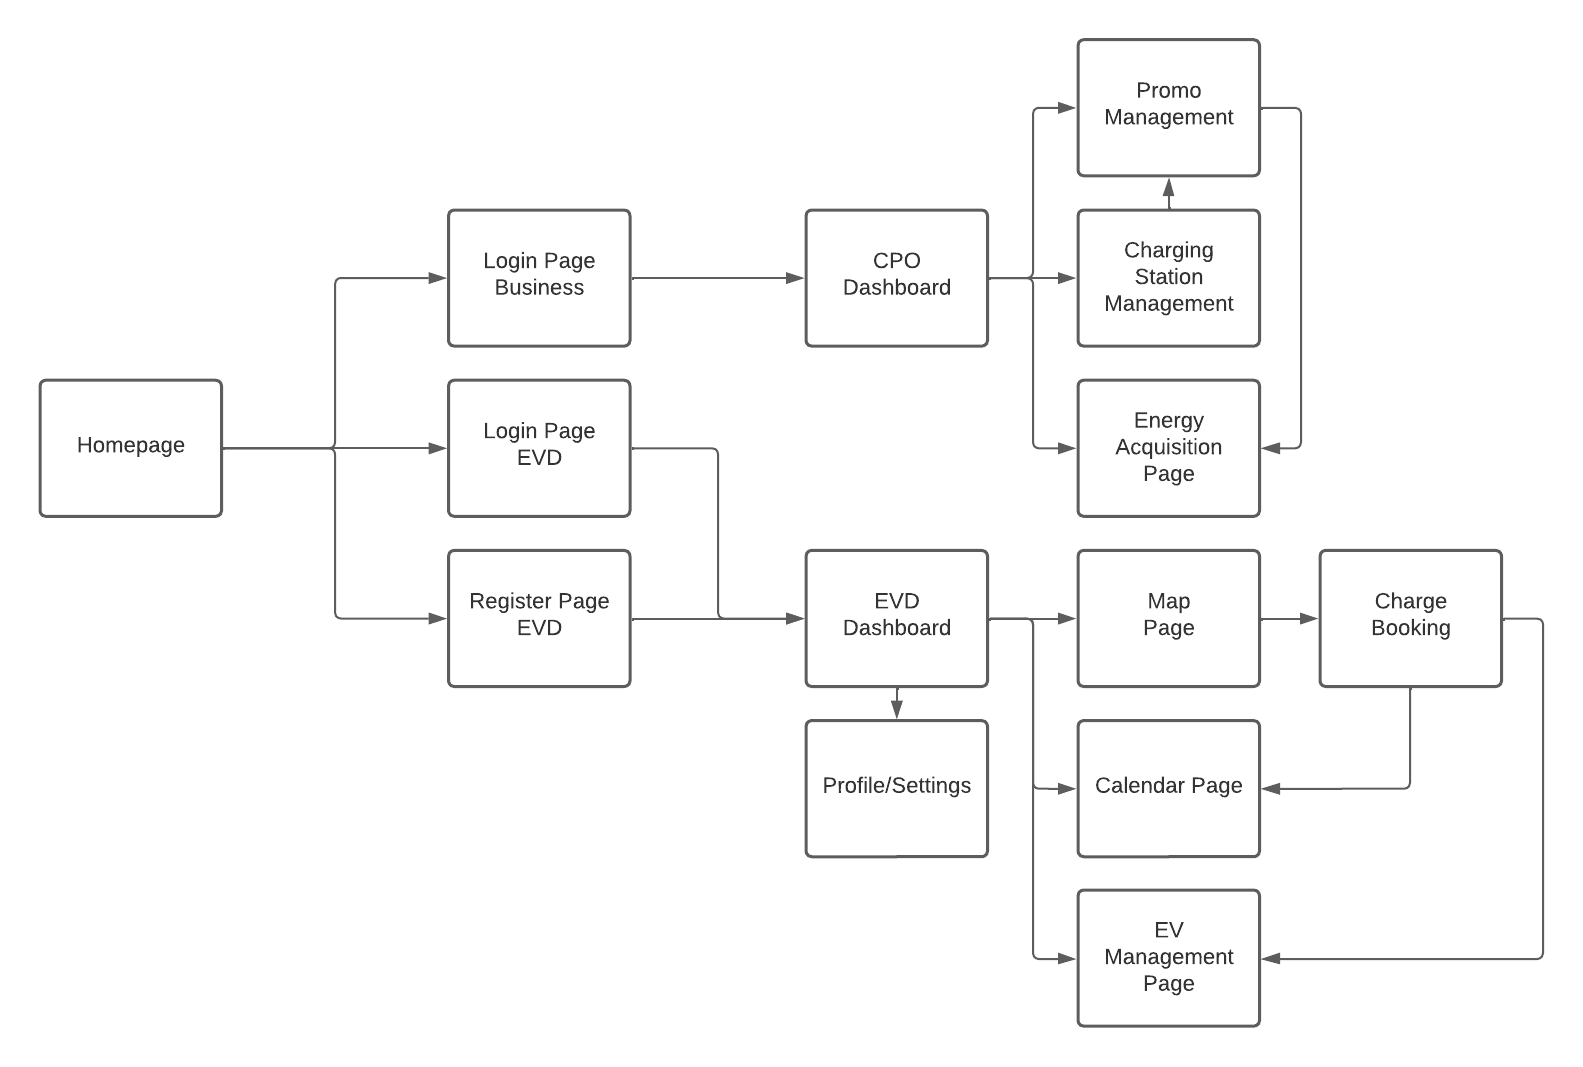
\includegraphics[width=1\linewidth]{UI/Pages}
        \caption{Pages of the eMALL system}
        \label{fig: pages}
    \end{center}
\end{figure}

We’ll also skip the homepage interface, as it is linked to marketing choices (colors, fonts, style) which are neither relevant nor functional to the description of the service.

As previously mentioned, the login section allows you to redirect the user, obviously following a successful login, to the dashboard from which you can access the service and take advantage of its features.
There are two types of dashboards, as are two actors involved in the eMALL processes: CPO, and registered EVD, who access the service via two different login pages, one reserved for the public (EVDs), one reserved for CPOs.

The CPO dashboard is aesthetically different from the EVD dashboard in the choice of colors, but maintains an almost identical structure in order to optimize and simplify its development, which can be reduced to the definition of a few reusable components, following an industrial, scalable design method and easily maintainable over time.

From the CPOs dashboard the following pages can be accessed:

\begin{itemize}
    \item Promo and offers management
    \item Charging stations management
    \item Energy acquisition management (interface with DSO offers)
\end{itemize}

From the EVDs dashboard the following pages can be accessed:

\begin{itemize}
    \item User profile and settings management
    \item Map of charging stations
    \item User’s calendar and appointments booked
    \item Owned EVs management
    \item Booking charge
\end{itemize}

It is also possible to receive targeted notifications for the user.
All the pages illustrated above are described in detail in the following pages.

Any interactive panels and dialogs are neglected in the development of the presented interface.

\begin{figure} [H]
    \begin{center}
        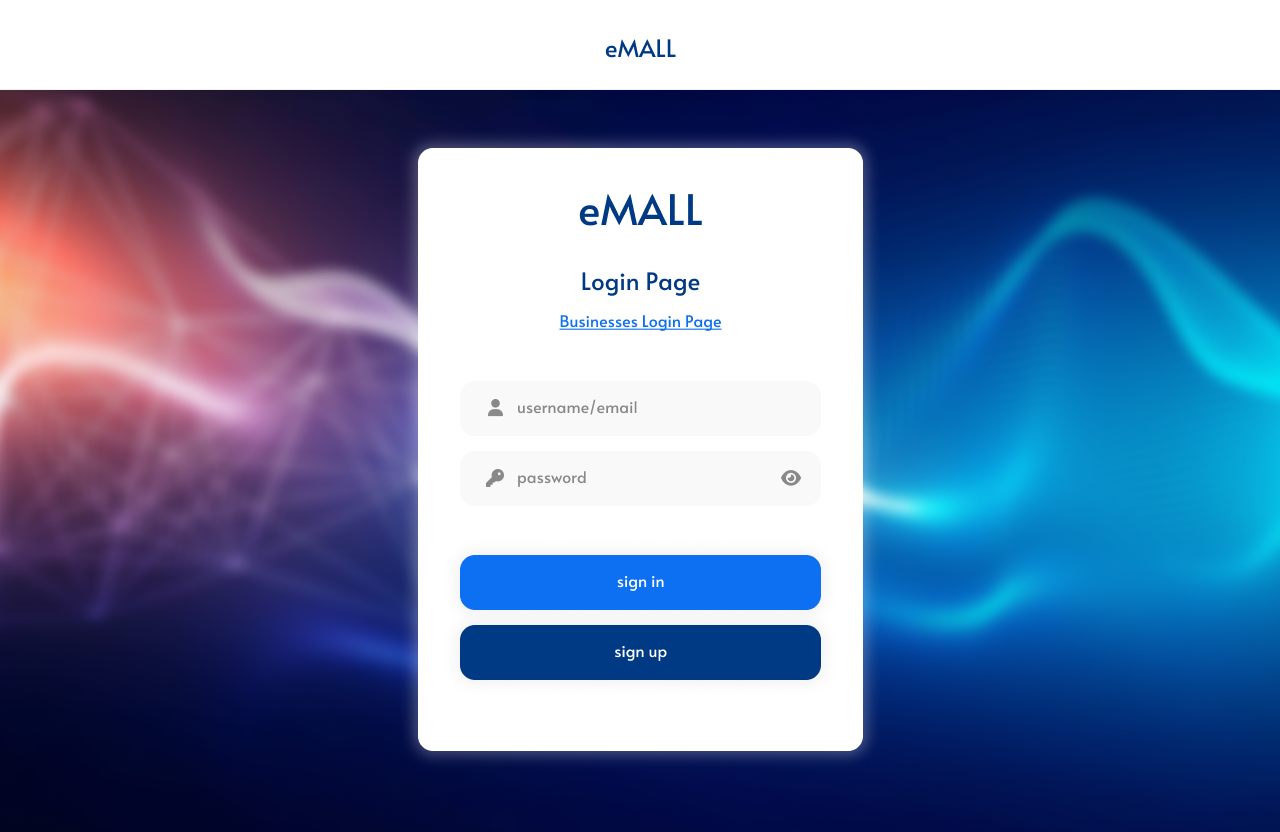
\includegraphics[width=1\linewidth]{UI/Signin}
        \caption{Login Page}
        \label{fig: signin}
    \end{center}
\end{figure}

\begin{figure} [H]
    \begin{center}
        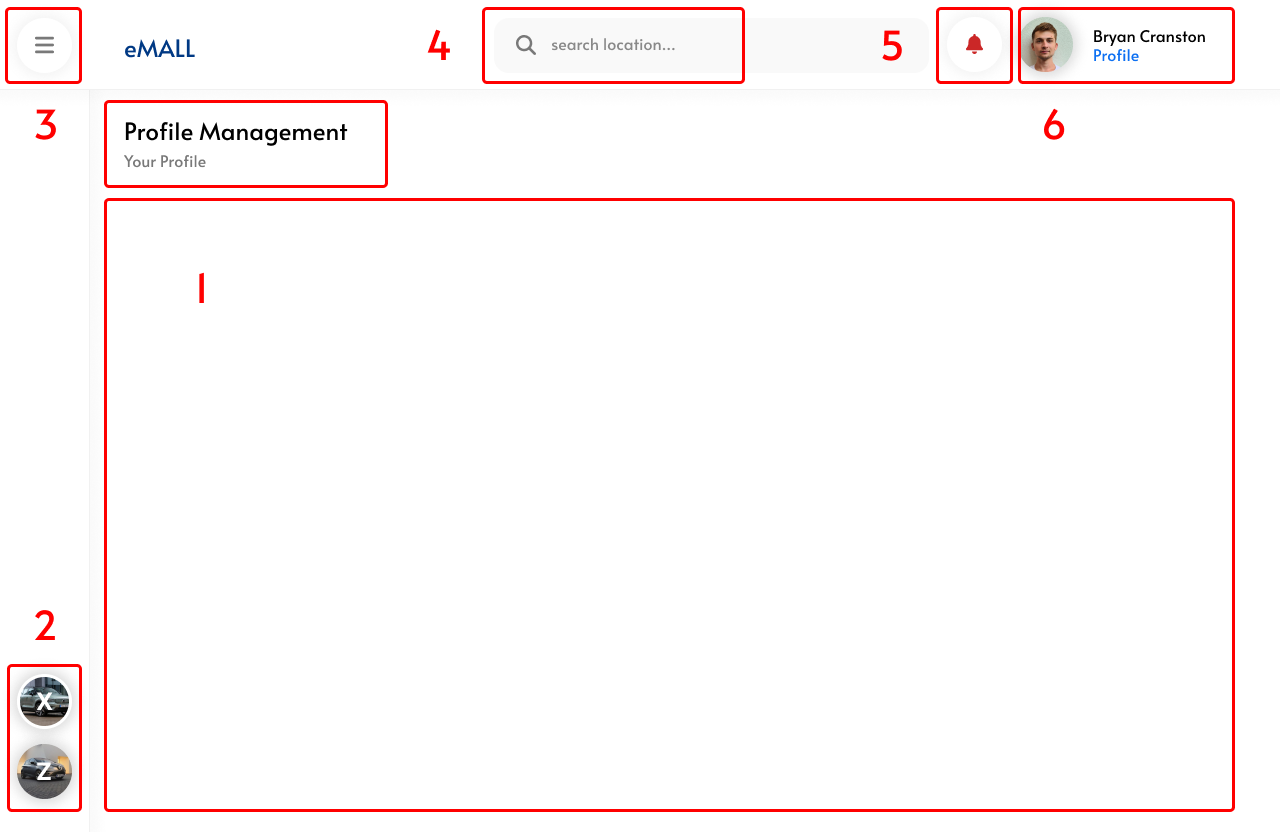
\includegraphics[width=1\linewidth]{UI/Wireframe}
        \caption{Wireframe of sticky bars}
        \label{fig: wireframe}
    \end{center}
\end{figure}

\begin{enumerate}
    \item \textbf{Main section:} contains the page
    \item \textbf{EV fast selector:} list buttons containing the EV owned by the user (only in the EVD dashboard), and highlights the selected EV
    \item \textbf{Hamburger toggle:} shows a menu with functions/pages offered by the system
    \item \textbf{Search bar:} permits to search a location and redirect to the map page with information about charging stations nearby
    \item \textbf{Notification bar:} contains notifications received by the user
    \item \textbf{Profile button:} redirects to the profile page
\end{enumerate}


\section{EVD Interface}
\label{sec: evd_interface}%
The EVD dashboard collects useful information for driver, everything at a glance.
The framework is designed to be modular, which makes it versatile and responsive.
The UI below contains some modules that could eventually be displayed;
the dashboard is thought in particular with a section dedicated to statistics, allowing users to view their charging stats and make the system smart.

\begin{figure} [H]
    \begin{center}
        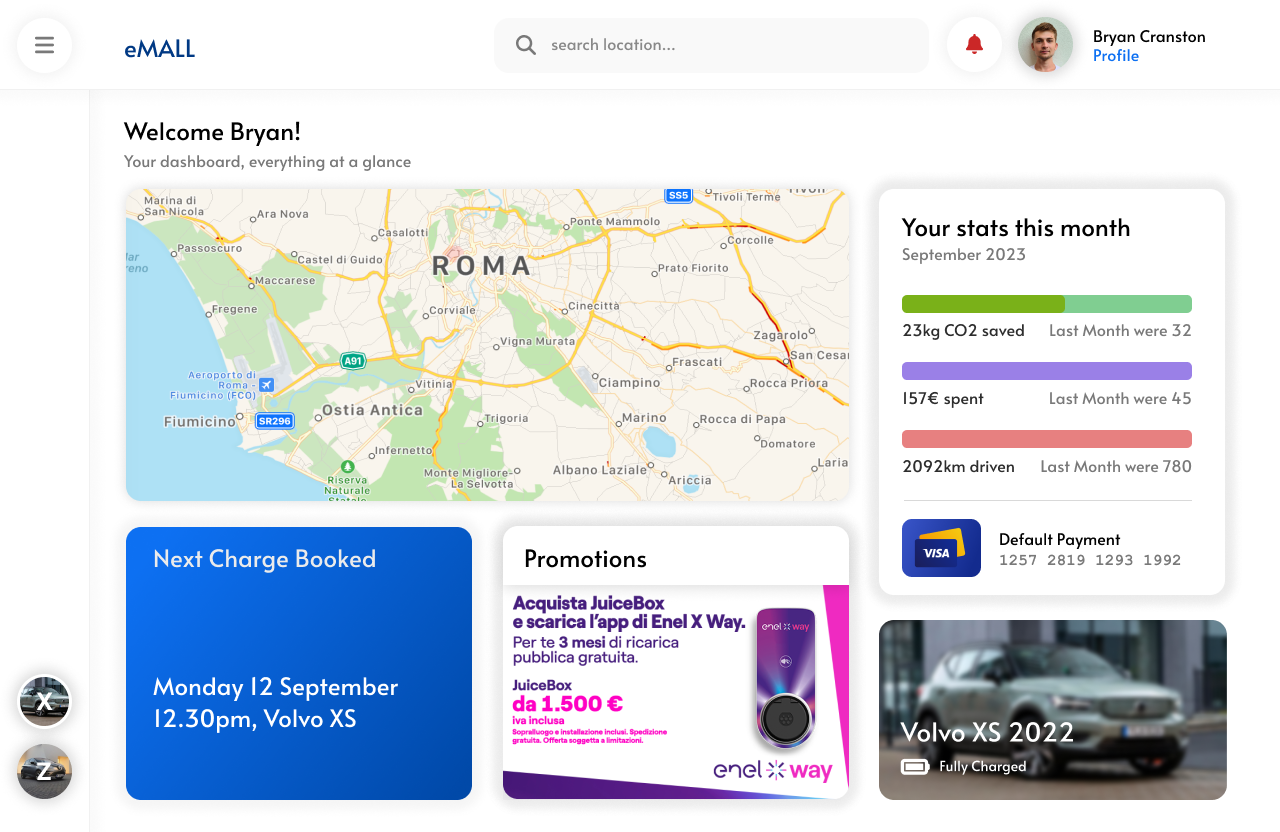
\includegraphics[width=1\linewidth]{UI/EVDDashboard}
        \caption{EVD Dashboard}
        \label{fig: evddashboard}
    \end{center}
\end{figure}

The process of booking a charge could begin looking at the map page, which is reported below.
The EVD can move around, and look for a charging stations that suits its requirements;

\begin{figure} [H]
    \begin{center}
        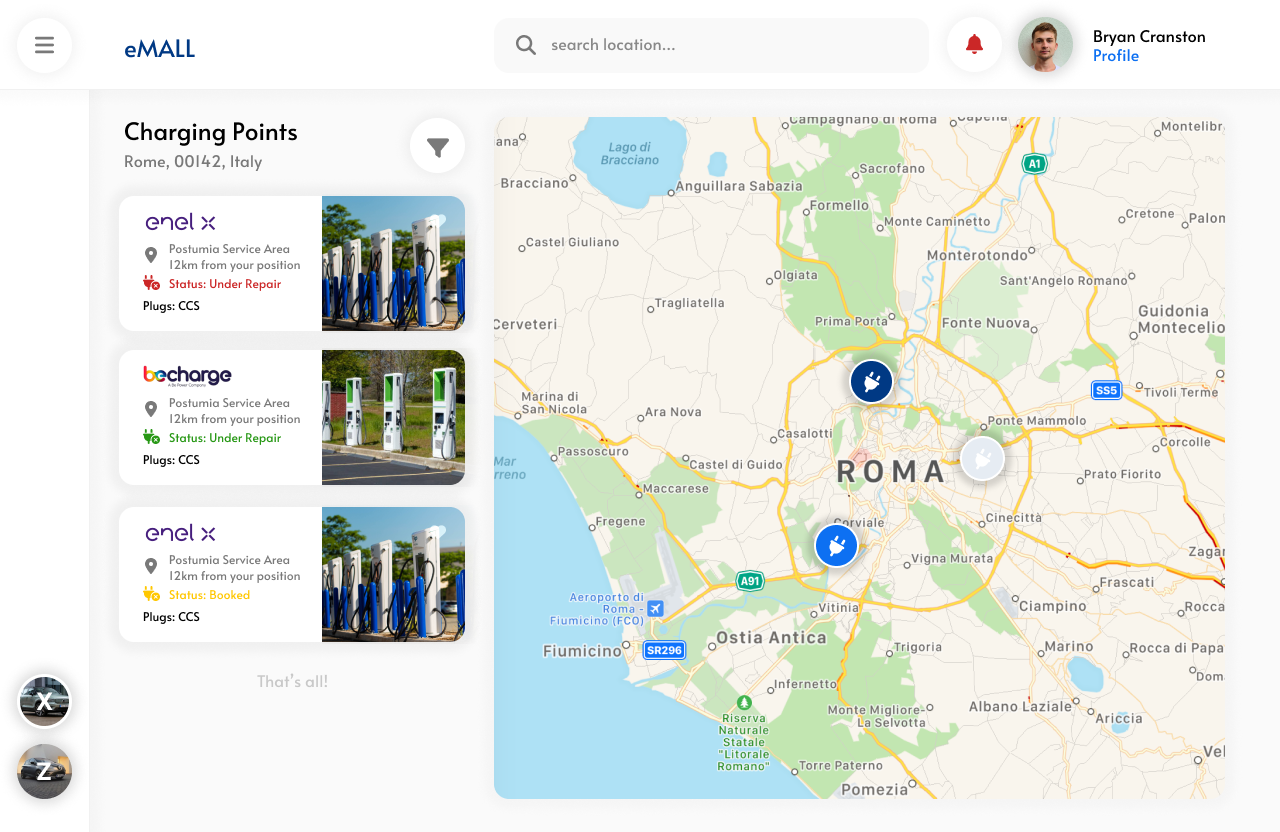
\includegraphics[width=1\linewidth]{UI/Map}
        \caption{Map page}
        \label{fig: map}
    \end{center}
\end{figure}

Once the choice has been made, the user is redirected to the booking section, containing a calendar showing the hourly availability of the columns and their status.
Some additional info about the charging stations are shown too.
The charge can be booked for a specific car, and a special button is provided right below the hourly table.
A user can explore the table, change dates, and confirm booking, or go back to the previous page.
Lastly, the EVD can add the charging station to its favorites.

\begin{figure} [H]
    \begin{center}
        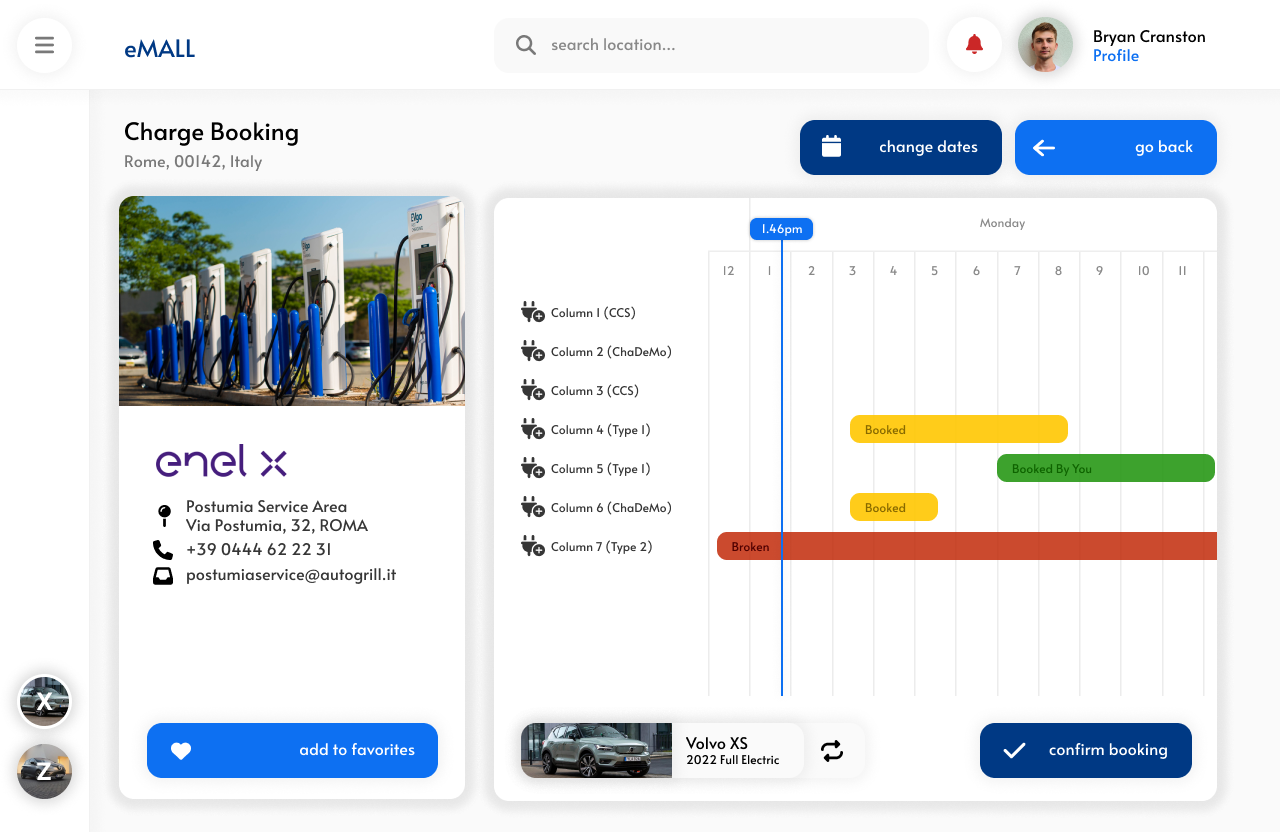
\includegraphics[width=1\linewidth]{UI/Chargebooking}
        \caption{Charge booking page}
        \label{fig: chargebooking}
    \end{center}
\end{figure}

From the dashboard or the menu, the EVD can access to its calendar, showing its appointments, and eventually any suggested charge, based on the EVD’s habits and its EV’s necessities.

\begin{figure} [H]
    \begin{center}
        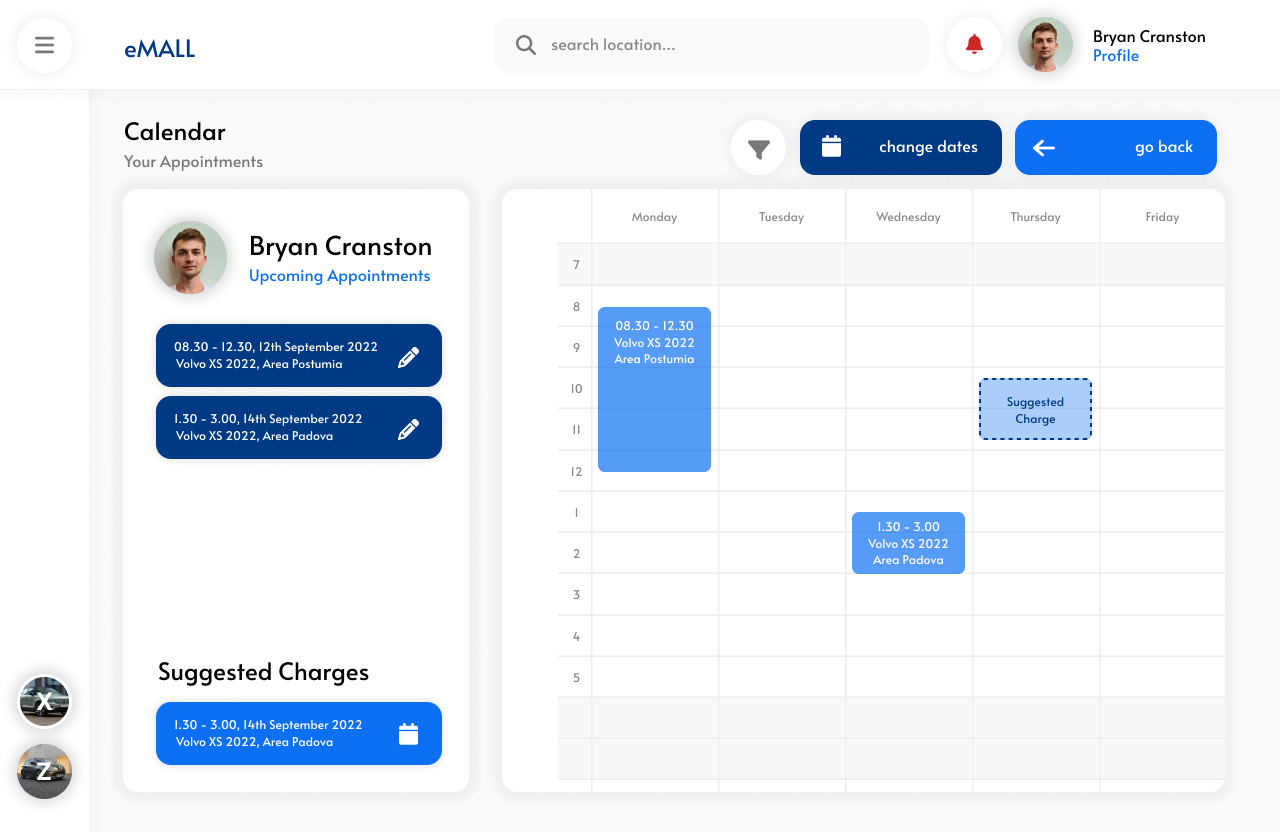
\includegraphics[width=1\linewidth]{UI/Calendar}
        \caption{Calendar page}
        \label{fig: calendar}
    \end{center}
\end{figure}

A user can update its EVs’ info, add new EV or remove them in the EV management section.

\begin{figure} [H]
    \begin{center}
        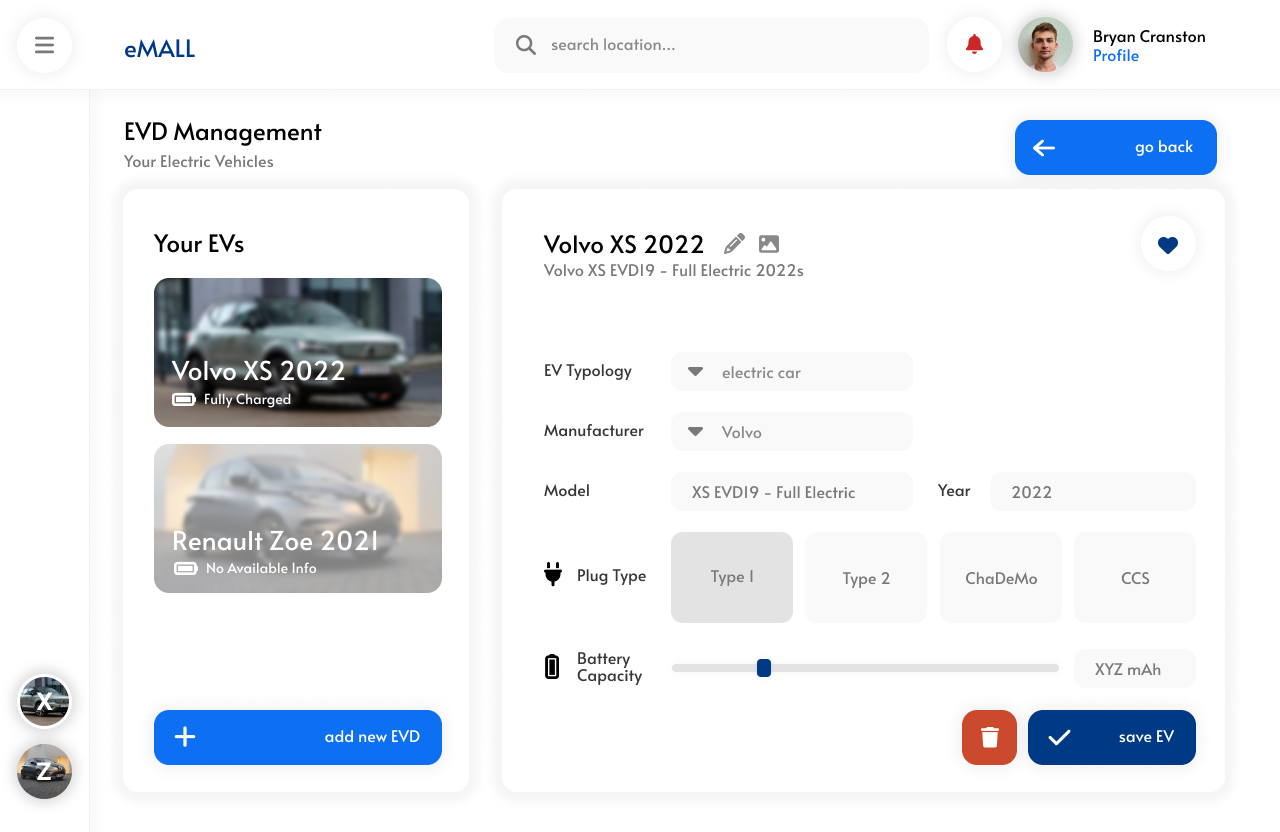
\includegraphics[width=1\linewidth]{UI/VM}
        \caption{EV Management page}
        \label{fig: vm}
    \end{center}
\end{figure}

Finally, a profile management section can be accessed from the profile button, or from the menu.
It contains information about the user, included billing address, and payment methods.

\begin{figure} [H]
    \begin{center}
        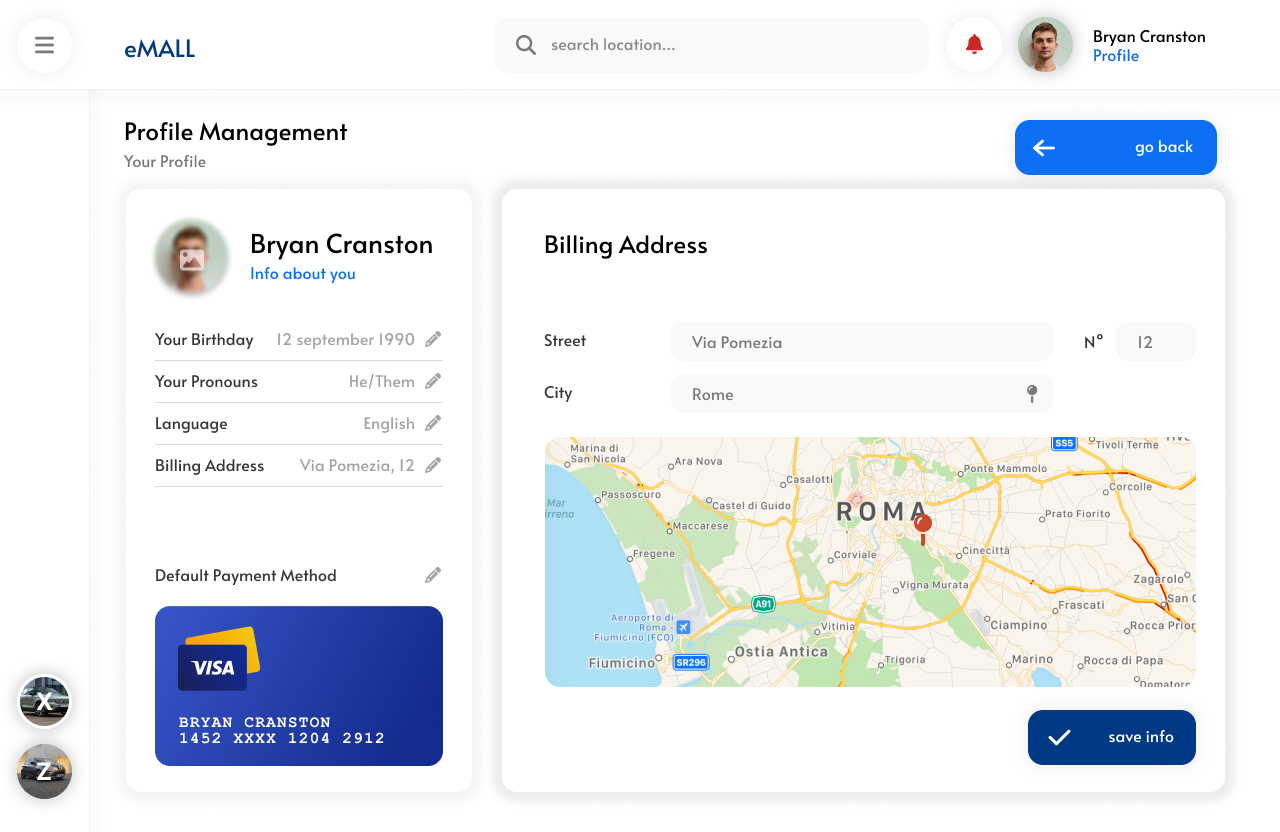
\includegraphics[width=1\linewidth]{UI/Settings}
        \caption{Settings page}
        \label{fig: settings}
    \end{center}
\end{figure}


\section{CPO Interface}
\label{sec: cpo_interface}%

The CPO’s interface is slightly different from the EVD’s interface, as said before.
Offered functions and pages are the charging station management page that is shown below, containing info about its location, and the status about charging points in the selected charging station.
The CPO’s operator can set fees, modify promo associated to a specific charging point, check DSO status, and finally save updated info.

\begin{figure} [H]
    \begin{center}
        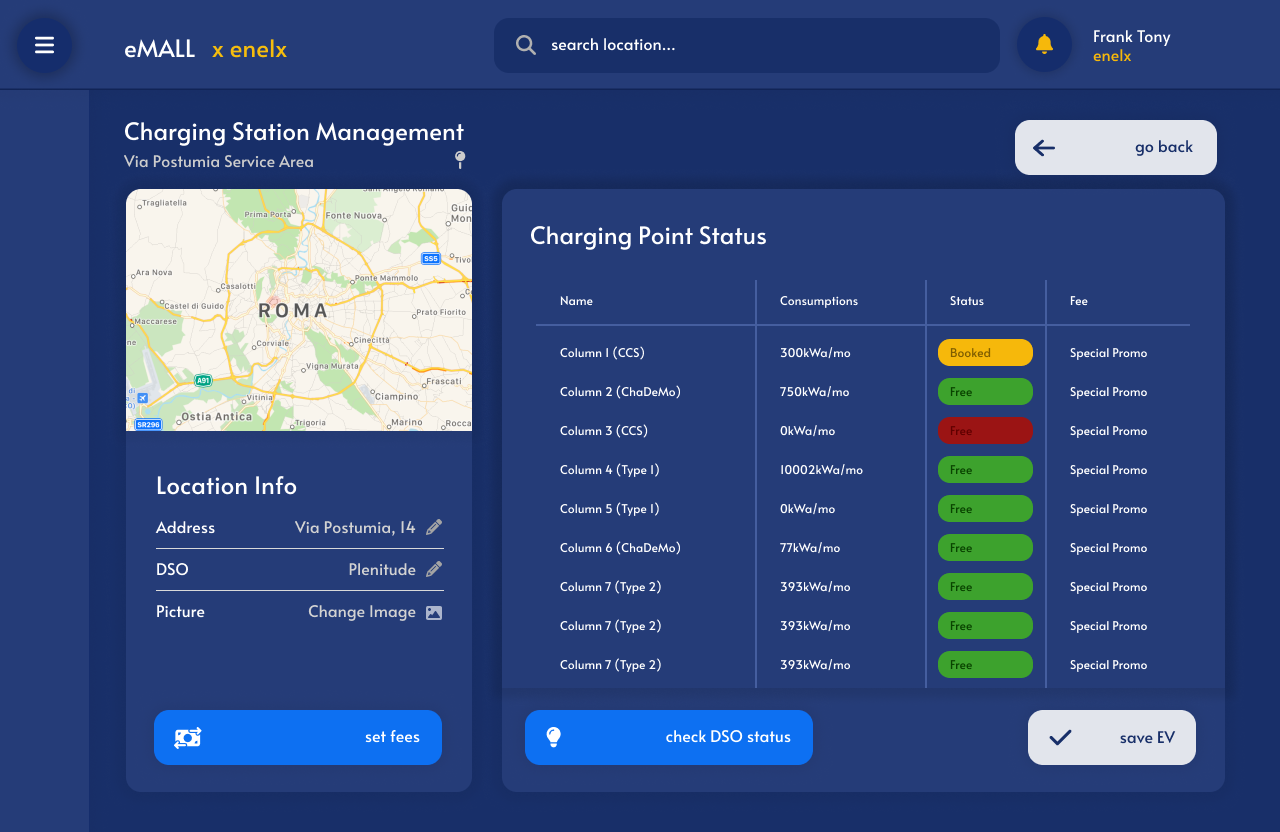
\includegraphics[width=1\linewidth]{UI/CSmgmt}
        \caption{Charging Station Management page}
        \label{fig: csmgmt}
    \end{center}
\end{figure}

The energy acquisition page is thought to be an interface with DSOs. It displays DSO (paused, used in the past, and active);
an overview is shown in the right module, containing information about the battery/energy used;
a log can be downloaded, to obtain more accurate information.
Stats about battery usage are shown in the right module too.

\begin{figure} [H]
    \begin{center}
        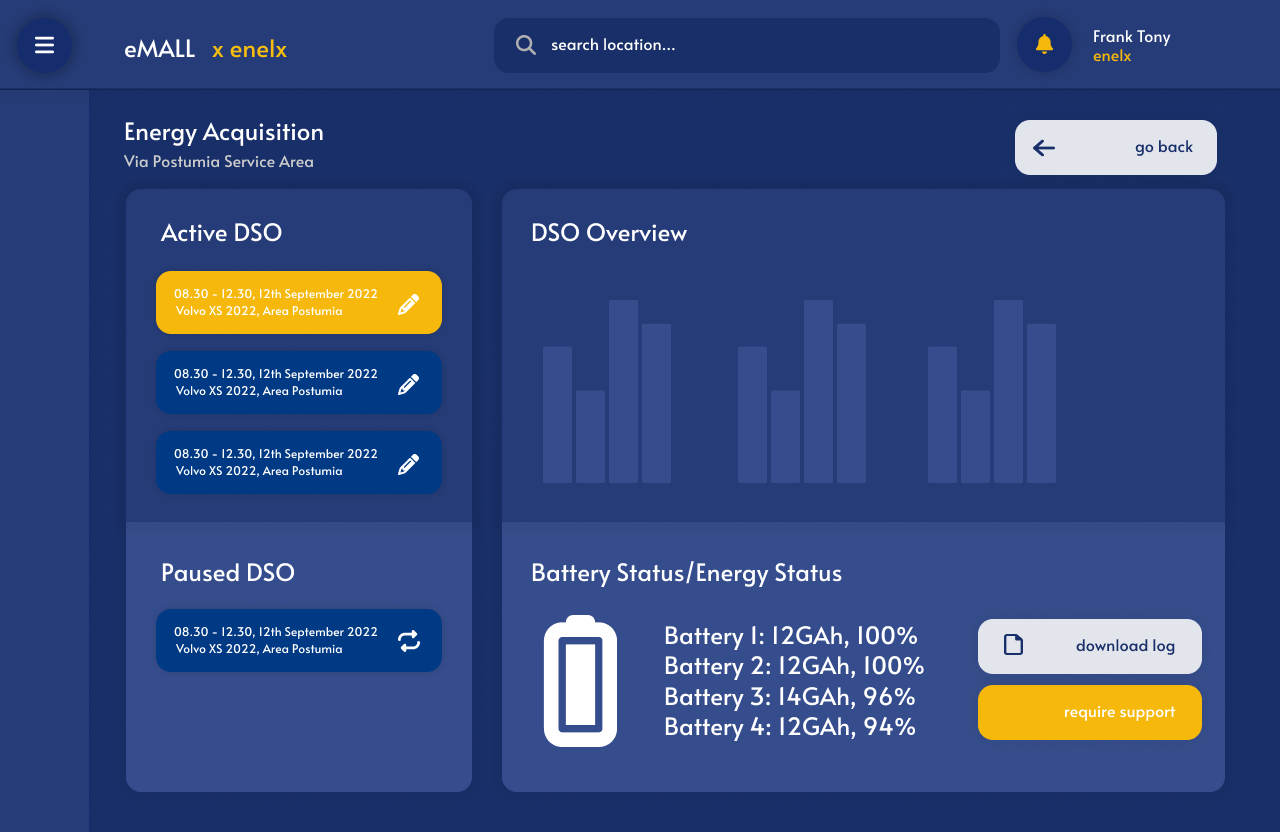
\includegraphics[width=1\linewidth]{UI/EA}
        \caption{Energy Acquisition Management page}
        \label{fig: ea}
    \end{center}
\end{figure}

Fees can be set, modified and eliminated in the fee management page.

\begin{figure} [H]
    \begin{center}
        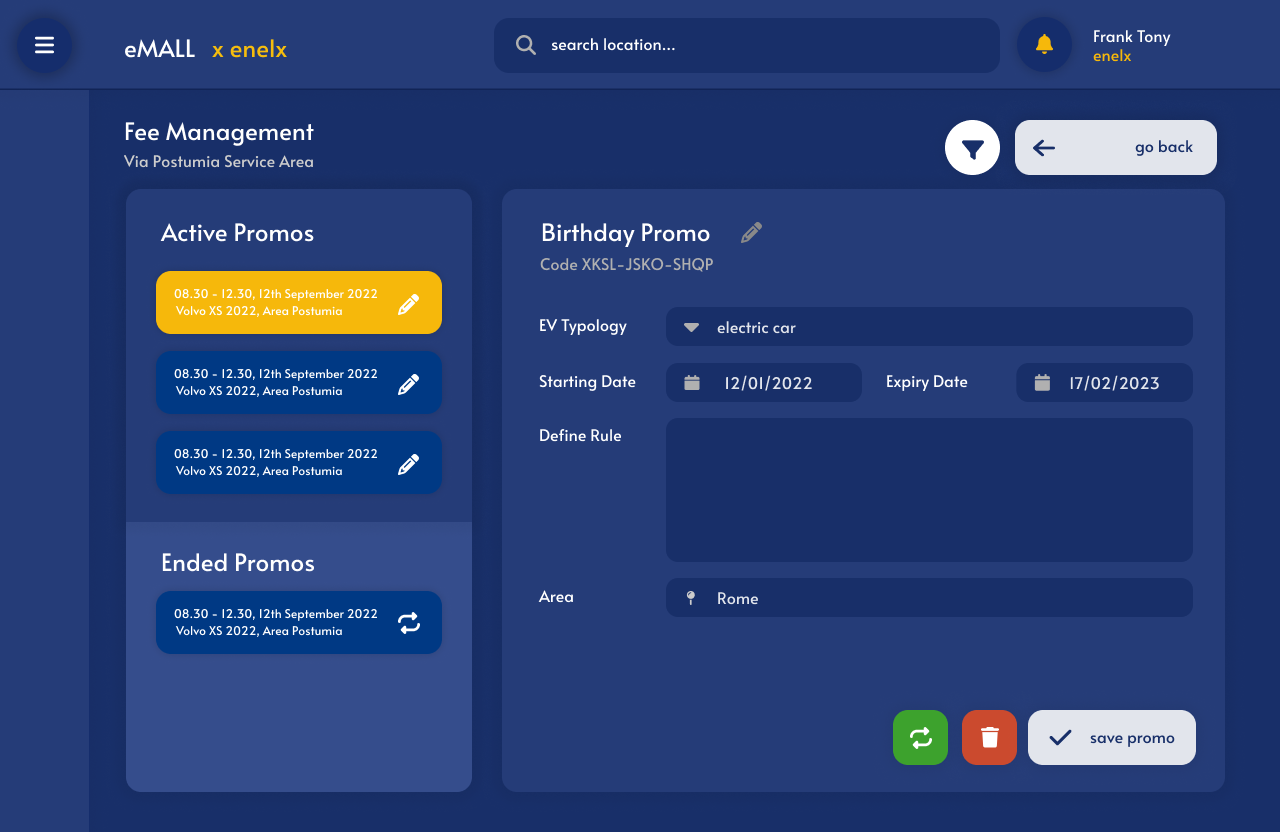
\includegraphics[width=1\linewidth]{UI/Promomgmt}
        \caption{Promo Management page}
        \label{fig: promomgmt}
    \end{center}
\end{figure}


    \chapter{Requirements Traceability}
    \label{ch:requirements_traceability}%
    This chapter shows how the functional and non-functional requirements of the eMALL system described in the RASD are met.
Firstly, we describe the mapping between the requirements listed in the 3.2.1 \textit{Requirements} section in the RASD
and the components identified in section 2.2 of this document.
Then, we comment on how \textit{Performance Requirements} and \textit{Software System Attributes} described in the 3.3
and 3.5 sections of the RASD are met thanks to the design adopted for the eMALL system.


\section{Functional Requirements Traceability}
\label{sec: functional_requirements_traceability}%
The following table lists all the requirements that are satisfied by the components.
Texts of the requirements are inserted in the table to facilitate comprehension.
\begin{center}
    \begin{longtable}{p{0.3\linewidth}p{0.7\linewidth}}
        \hline
        Registration Service                   & R1. The eMALL system shall allow an unregistered EVD to create an account.                                                                      \\
        & R69.\ The eMALL system shall store users information.                                                                                           \\
        \hline
        EVD Authentication Service             & R2. The eMALL system shall allow a registered EVD to log in.                                                                                    \\
        \hline
        EVD Profile Manager Service            & R3. The eMALL system shall allow a registered EVD to add an EV in his profile.                                                                  \\
        & R21.\ The eMALL system shall allow a registered EVD to insert a new payment method.                                                             \\
        & R22.\ The eMALL system shall allow a registered EVD to select a payment method.                                                                 \\
        & R69.\ The eMALL system shall store users information.                                                                                           \\
        \hline
        Explore Stations Service               & R8. The eMALL system shall allow a registered EVD to get all the charging station near to his current location.                                 \\
        & R9. The eMALL system shall allow a registered EVD to insert a specific location to get charging station nearby.                                 \\
        & R10.\ The eMALL system shall allow a registered EVD to move into the map of charging stations.                                                  \\
        & R11.\ The eMALL system shall allow a registered EVD to select a specific charging station.                                                      \\
        & R12.\ The eMALL system shall allow a registered EVD to get the location of a specific charging station.                                         \\
        & R13.\ The eMALL system shall allow a registered EVD to get the costs of a specific charging station.                                            \\
        & R14.\ The eMALL system shall allow a registered EVD to get the CPO owner of a specific charging station.                                        \\
        & R15.\ The eMALL system shall allow a registered EVD to get type of connectors of a specific charging station.                                   \\
        & R16.\ The eMALL system shall allow a registered EVD to get maximum power supply of the spots of a specific charging station.                    \\
        & R17.\ The eMALL system shall allow a registered EVD to get the status of a specific charging station.                                           \\
        \hline
        Booking Service                        & R5. The eMALL system shall allow a registered EVD to book a charge.                                                                             \\
        & R6. The eMALL system shall allow a registered EVD to select a timeframe to reserve a charging point.                                            \\
        & R55.\ The eMALL system shall reserve a charging point in a certain timeframe.                                                                   \\
        & R69.\ The eMALL system shall store users information.                                                                                           \\
        \hline
        Manage Charging Session Service        & R25.\ The eMALL system shall allow a registered EVD to start a charging process.                                                                \\
        & R26.\ The eMALL system shall verify the identity of the EVD requesting to start a charging session.                                             \\
        & R32.\ The eMALL system shall send notifications about the current status of the charging session to the registered EVD.                         \\
        & R33.\ The eMALL system shall allow a registered EVD to stop the charging session.                                                               \\
        & R35.\ The eMALL system shall send the receipt of the charging session to the registered EVD.                                                    \\
        & R69.\ The eMALL system shall store users information.                                                                                           \\
        \hline
        Promotion Service                      & R18.\ The eMALL system shall allow a registered EVD to get the list of active promotions.                                                       \\
        & R19.\ The eMALL system shall allow a registered EVD to select a specific promotion.                                                             \\
        & R20.\ The eMALL system shall allow a registered EVD to activate a promotion.                                                                    \\
        \hline
        Calendar Service                       & R7. The eMALL system shall add a booked reservation into EVD’s calendar.                                                                        \\
        & R37.\ The eMALL system shall allow a registered EVD to access in his own calendar.                                                              \\
        & R38.\ The eMALL system shall allow a registered EVD to add a new activity into his calendar.                                                    \\
        & R39.\ The eMALL system shall allow a registered EVD to specify the starting hour of a new activity.                                             \\
        & R40.\ The eMALL system shall allow a registered EVD to specify the destination of a new activity.                                               \\
        & R41.\ The eMALL system shall save a new activity into EVD’s calendar.                                                                           \\
        & R69.\ The eMALL system shall store users information.                                                                                           \\
        \hline
        Suggestion Service                     & R4. The eMALL system shall communicate with EV’s brand API to get needed information.                                                           \\
        & R42.\ The eMALL system shall calculate the best schedules of where and when to charge registered EVD’s EV so to minimize costs and wasted time. \\
        & R43.\ The eMALL system shall communicate to the registered EVD the details of the suggestions about the calculated schedules.                   \\
        \hline
        Payment Service                        & R23.\ The eMALL system shall allow a registered EVD to pay with the preferred payment method.                                                   \\
        & R24.\ The eMALL system shall communicate with third-party payment services to make the payments.                                                \\
        & R36.\ The eMALL system shall communicate the outcome of the payment to a registered EVD.                                                        \\
        \hline
        CPO Authentication Service             & R44.\ The eMALL system shall allow a CPO to log in as a business user.                                                                          \\
        &                                                                                                                                                 \\
        \hline
        CPO Profile Manager Service            & R66.\ The eMALL system shall allow a CPO to update its electricity provider.                                                                    \\
        & R69.\ The eMALL system shall store users information.                                                                                           \\
        & R70.\ The eMALL system shall allow the CPO to manage its company personal information.                                                          \\
        \hline
        Charging Station Manager Service       & R45.\ The eMALL system shall allow a CPO to manage its charging stations.                                                                       \\
        & R46.\ The eMALL system shall allow a CPO to set new selling prices for charging sessions.                                                       \\
        & R47.\ The eMALL system shall allow a CPO to add a new charging station in its profile.                                                          \\
        & R48.\ The eMALL system shall allow a CPO to specify the location of charging station (region, province, city, address).                         \\
        & R49.\ The eMALL system shall allow a CPO to specify the status of a charging station (available, maintenance, broken, unavailable).             \\
        & R50.\ The eMALL system shall allow a CPO to add a charging point in an existing charging station.                                               \\
        & R51.\ The eMALL system shall allow a CPO to specify the serial number of charging point.                                                        \\
        & R52.\ The eMALL system shall allow a CPO to specify the types of connectors of a charging point.                                                \\
        & R53.\ The eMALL system shall allow a CPO to specify the maximum power of a charging point.                                                      \\
        & R54.\ The eMALL system shall allow a CPO to specify the type of connectors of a charging point.                                                 \\
        & R61.\ The eMALL system shall allow a CPO to schedule a maintenance session for a charging station.                                              \\
        & R62.\ The eMALL system shall allow a CPO to specify date and starting hour of a maintenance session for a charging station.                     \\
        & R69.\ The eMALL system shall store users information.                                                                                           \\
        \hline
        Charging Station Communication Service & R28.\ The eMALL system shall communicate to charging points to start the charging session.                                                      \\
        & R29.\ The eMALL system shall define the source of the charging session (batteries or DSO).                                                      \\
        & R30.\ The eMALL system shall define the power of the charging session.                                                                          \\
        & R31.\ The eMALL system shall get EV’s battery status.                                                                                           \\
        & R34.\ The eMALL system shall communicate to a charging point to stop the charging session.                                                      \\
        & R63.\ The eMALL system shall communicate to a charging station to schedule a maintenance at a specified timeframe.                              \\
        \hline
        Promotion Manager Service              & R56.\ The eMALL system shall allow a CPO to manage its promotions.                                                                              \\
        & R57.\ The eMALL system shall allow a CPO to create a new promotion.                                                                             \\
        & R58.\ The eMALL system shall allow a CPO to specify the details of the a promotion.                                                             \\
        & R59.\ The eMALL system shall save the information of a promotion.                                                                               \\
        & R60.\ The eMALL system shall initialize the information of a new promotion.                                                                     \\
        \hline
        DSO Manager Service                    & R64.\ The eMALL system shall allow a CPO to get the list of DSOs.                                                                               \\
        & R65.\ The eMALL system shall allow a CPO to select a DSO from the list of DSOs.                                                                 \\
        & R67.\ The eMALL system shall communicate to a specified DSO to send energy to the charging stations of a CPO.                                   \\
        & R68.\ The eMALL system shall get the electricity selling prices from the DSOs.                                                                  \\
        \hline
        \caption{Mapping between components and requirements.}
        \label{tab: map_comp_req}%
    \end{longtable}
\end{center}


\section{Non Functional Requirements Traceability}
\label{sec: non_functional_requirements_traceability}%

\subsection{Performance Requirements}
\label{subsec:performance_requirements}%
The \textit{Number of users} section (3.3 of the RASD) says that the system should be able to handle $50\ 000$ users.
The performance requirement is guaranteed thanks to the adopted of a microservices architecture and
the insertion of a load balancer to distribute requests into the several nodes that constitute the system.
In this way, the system avoids cases of network congestion. \\
From the time response point of view, there are not strict performance requirements.
According to the relations explained in the previous sections, there are not complex communications, so the time needed
by the \verb|eMALL| system to answer to received requests won't be high.

\subsection{Software System Attributes}
\label{subsec:software_system_attributes}%
Thanks to loose coupling considered for the identification of services, when a module fails the rest of the system keeps running.
In this way, the availability of the system is guaranteed.
When a module fails, it is not necessary to halt the whole system to proceed with the maintenance session:
only the service in question will be maintained, the other ones won't be influenced.
Finally, the system guarantees security for users information encrypting them before proceeding with the storage
and memorizing all the data on the server side.
The client, as already explained in the 2.7.3 section will be a thin client, so its purpose is to communicate with services
interfaces and sending requests to the server, that will handle any insertion, update or deletion of data.


    \chapter{Implementation, Integration and Test Plan}
    \label{ch:implementation_integration_test_plan}%
    \section{Implementation \& Integration}
\label{sec: implementation}%
As showed in the deployment diagram, there relations between services that should be considered for the definition of
the order of implementation of the modules.
We suppose that DBMS are already deployed systems that will be used by our components.
It follows a list of a possible path for the implementation.
Each step lists modules that can be deployed in parallel.
The order is defined by the dependencies between components.
It is:
\begin{itemize}
    \item We start with the modules that directly communicate with DBMSs. They are: Registration Service,
    EVD Authentication Service, EVD Profile Manager Service, Explore Stations Service, Calendar Service, CPO Authentication Service,
    CPO Profile Manager Service, Charging Stations Manager Service.
    \item The implementation should continue with modules that allow communication with external services.
    They are: Payment Service, Charging Station Communication Service, DSO Manager Service.
    \item Now it is the turn of components that have strong relations with previous implemented service, as:
    Promotion Service, Booking Service and Charging Session Service.
    \item Finally, it has to be implemented the module that communicates with the greater number of services: Suggestion Service.
    In this final step, it should be completed the process for the asynchronous call started by Calendar Service
    after the addition of a new activity.
\end{itemize}


\section{Test Plan}
\label{sec: test_plan}%
\subsection{Functional Testing}
The system should be tested in order to actually guarantee the functionalities described in the RASD document; this can be done executing automated tests.
Performances should be checked too, and this can be done simulating real life scenarios in a real world environment, stressing the system.
\subsection{User Interface Testing}
Regarding the UI/UX, as said in the RASD document, it is crucial that the application is intuitive and as easy to use as possible, since it will be fruited by elderly and users that will be not always practical with new electronic services; to achieve this goal, the user experience will have to be tested focusing on features such as usability and accessibility. Focus groups, composed by old persons and digital non-natives, could test the journey through the app, in order to test its smoothness. Automated tests could be conducted to test scenarios described in the RASD document.


    \chapter{Effort Spent}
    \label{ch:effort_spent}%
    \begin{table}[H]
    \begin{center}
        \begin{tabular}{c|c}
            \hline
            Member of group & Effort spent \\
            \hline
            Cela Irfan & \begin{tabular}{p{0.5\linewidth}|c}
                             Introduction                              & $3h$  \\
                             Architectural Design                      & $29h$ \\
                             User Interface Design                     & $0h$  \\
                             Requirements Traceability                 & $0h$  \\
                             Implementation, Integration and Test Plan & $0h$  \\
                             Reasoning                                 & $8h$  \\
            \end{tabular} \\
            \hline
            Cela Mario & \begin{tabular}{p{0.5\linewidth}|c}
                             Introduction                              & $h$ \\
                             Architectural Design                      & $37h$ \\
                             User Interface Design                     & $h$ \\
                             Requirements Traceability                 & $5h$ \\
                             Implementation, Integration and Test Plan & $h$ \\
                             Reasoning                                 & $h$ \\
            \end{tabular} \\
            \hline
            Cogollo Alessandro & \begin{tabular}{p{0.5\linewidth}|c}
                                     Introduction                              & $h$ \\
                                     Architectural Design                      & $h$ \\
                                     User Interface Design                     & $h$ \\
                                     Requirements Traceability                 & $h$ \\
                                     Implementation, Integration and Test Plan & $h$ \\
                                     Reasoning                                 & $h$ \\
            \end{tabular} \\
            \hline
        \end{tabular}
        \caption{Effort spent by each member of the group.}
        \label{tab:effor_spent}
    \end{center}
\end{table}

    \chapter{References}
    \label{ch:references}%
    \section{Paper References}
\label{sec: paper_references}%


\section{Used Tools}
\label{sec: used_tools}%


% LIST OF FIGURES
    \listoffigures

% LIST OF TABLES
    \listoftables
    \cleardoublepage
\end{document}
